\documentclass{article}
%%%%%%%%%%%%%%%%%%%%%%%%%%%%%%%%%%%%%%%%%%%%%%%%%%%%%%
% Math
%%%%%%%%%%%%%%%%%%%%%%%%%%%%%%%%%%%%%%%%%%%%%%%%%%%%%%
\usepackage{amsmath}
\usepackage{amssymb}
\usepackage{amsfonts} %para usar as fontes %matematicas, e pega fontes para \mathbb
\usepackage{amsthm}   %ambientes com teoremas (usar depois de amsmath)
%\usepackage{biblatex}
%\usepackage{natbib}

%%%%%%%%%%%%%%%%%%%%%%%%%%%%%%%%%%%%%%%%%%%%%%%%%%%%%%
%Graphs
%%%%%%%%%%%%%%%%%%%%%%%%%%%%%%%%%%%%%%%%%%%%%%%%%%%%%%
\usepackage{graphics}
\usepackage{graphicx}
\usepackage{texdraw}
\usepackage{color}
\usepackage{subfigure} 
\usepackage{tikz}
\usepackage[usenames,dvipsnames]{pstricks}
\usepackage{epsfig}
%\usepackage{pst-grad} % For gradients
%\usepackage{pst-plot} % For axes
%\usepackage{movie15}
\usepackage{animate}
\usetikzlibrary{decorations.fractals}
\usepackage{tikz}
%\usepackage{wrapfig}
\usepackage{pstricks}
\usepackage{multirow}
%%%%%%%%%%%%%%%%%%%%%%%%%%%%%%%%%%%%%%%%%%%%%%%%%%%%%%
% Format
%%%%%%%%%%%%%%%%%%%%%%%%%%%%%%%%%%%%%%%%%%%%%%%%%%%%%%
\usepackage[figurename=Fig.]{caption}
\usepackage[labelformat=empty]{caption}
\usepackage{gensymb}
\usepackage{cancel}
\usepackage{caption} % removing prefix from figure caption in LaTeX
\usepackage{subcaption}
\usepackage{url}
\usepackage{setspace}
%\usepackage{verbatim}
\usepackage{hyperref}
\usepackage{fancyhdr}
\usepackage{pgf}
\usepackage{lscape}
\usepackage{multicol}
%%%%%%%%%%%%%%%%%%%%%%%%%%%%%%%%%%%%%%%%%%%%%%%%%%%%%%
% Graphs path to the Picture Folder
%%%%%%%%%%%%%%%%%%%%%%%%%%%%%%%%%%%%%%%%%%%%%%%%%%%%%%
%\graphicspath{/home/henry/Desktop/UTEP_Proposal_Thesis/PhD_Thesis/Pictures}
\graphicspath{{Pictures/}{Data/}{References}} % Two folders Picture and Data    
%%%%%%%%%%%%%%%%%%%%%%%%%%%%%%%%%%%%%%%%%%%%%%%%%%%%%%
% page edition
%%%%%%%%%%%%%%%%%%%%%%%%%%%%%%%%%%%%%%%%%%%%%%%%%%%%%%
%\linespread{2.5}
\addtolength{\textwidth}{3cm}
\addtolength{\textheight}{3cm}
\addtolength{\hoffset}{-2cm}
% In case you need to adjust margins:
\topmargin=-0.5 in      %
\evensidemargin= .5 in     %
\oddsidemargin= .5 in      %
\textwidth = 7 in        %
\textheight = 9.0 in       %
\headsep = 0.15 in  
\pagestyle{fancyplain}
\lhead{\fancyplain{}{ROOFLINE MODEL - Spring 2021}}
\rhead{\fancyplain{}{Henry R. Moncada}}

%%%%%%%%%%%%%%%%%%%%%%%%%%%%%%%%%%%%%%%%%%%%%%%%%%%%%%
% Code Listing
% %%%%%%%%%%%%%%%%%%%%%%%%%%%%%%%%%%%%%%%%%%%%%%%%%%%%%%
 \usepackage[utf8]{inputenc}  % UTF-8 byte
\usepackage[T1]{fontenc}
\usepackage[variablett]{lmodern}% with proportional type writer font
\usepackage{pmboxdraw}
\usepackage{alltt}

\usepackage{listings}             % Include the listings-package
\usepackage{color}
\usepackage{xcolor}

\lstset{escapeinside={<@}{@>}}
\definecolor{codegreen}{rgb}{0,0.6,0}
\definecolor{codegray}{rgb}{0.5,0.5,0.5}
\definecolor{codepurple}{rgb}{0.58,0,0.82}
\definecolor{backcolour}{rgb}{0.95,0.95,0.92}
\lstset{
% BOX STYLE
  %aboveskip=3mm,
  %belowskip=3mm,  
  %frame=tb,
  frame=single,                    % adds a frame around the code  
% TEXT STYLE
  %basicstyle={\small\ttfamily},  
  basicstyle=\footnotesize,        % the size of the fonts that are used for the code
    %backgroundcolor=\color{white},   % choose the background color; you must add \usepackage{color} or \usepackage{xcolor}; should come as last argument
  breaklines=true,                 % sets automatic line breaking
  breakatwhitespace=true,          % sets if automatic breaks should only happen at whitespace
  %backgroundcolor=\color{lightgray},
  backgroundcolor=\color{backcolour},   
  commentstyle=\color{codegreen},    % comment style
  columns=flexible,   
  %deletekeywords={...},            % if you want to delete keywords from the given language
  %firstnumber=1000,                % start line enumeration with line 1000
  identifierstyle=\color{purple!60!black},
  keywordstyle=\color{blue},       % keyword style
  %language=Java,
  %language=bash,                   % the language of the code
  %numbers=none,
  numbers=left,                    % where to put the line-numbers; possible values are (none, left, right)
  %numberstyle=\tiny\color{codegray},  % the style that is used for the line-numbers
  numbersep=5pt,                   % how far the line-numbers are from the code
  stringstyle=\color{orange},       % string literal style
  showstringspaces=false,          % underline spaces within strings only
  %showspaces=false,                % show spaces everywhere adding particular underscores; it overrides 'showstringspaces'    
  %showtabs=false,                  % show tabs within strings adding particular underscores
  %stepnumber=2,                    % the step between two line-numbers. If it's 1, each line will be numbered
  tabsize=3                        % sets default tabsize to 2 spaces
  %                  % show the filename of files included with \lstinputlisting; also try caption instead of title 
}
%%%%%%%%%%%%%%%%%%%%%%%%%%%%%%%%%%%%%%%%%%%%%%%%%%%%%%
%listing tree
% %%%%%%%%%%%%%%%%%%%%%%%%%%%%%%%%%%%%%%%%%%%%%%%%%%%%%%
\lstdefinestyle{tree}{
    literate=
    {├}{{\smash{\raisebox{-1ex}{\rule{1pt}{\baselineskip}}}\raisebox{0.5ex}{\rule{1ex}{1pt}}}}1 
    {─}{{\raisebox{0.5ex}{\rule{1.5ex}{1pt}}}}1 
    {└}{{\smash{\raisebox{0.5ex}{\rule{1pt}{\dimexpr\baselineskip-1.5ex}}}\raisebox{0.5ex}{\rule{1ex}{1pt}}}}1 
  }
%%%%%%%%%%%%%%%%%%%%%%%%%%%%%%%%%%%%%%%%%%%%%%%%%%%%%%
%
% %%%%%%%%%%%%%%%%%%%%%%%%%%%%%%%%%%%%%%%%%%%%%%%%%%%%%%  
% \usepackage{lstlinebgrd} % The following patch fix the issue with lstlinebgrd
\makeatletter
\let\old@lstKV@SwitchCases\lstKV@SwitchCases
\def\lstKV@SwitchCases#1#2#3{}
\makeatother
\usepackage{lstlinebgrd}
\makeatletter
\let\lstKV@SwitchCases\old@lstKV@SwitchCases

\lst@Key{numbers}{none}{%
    \def\lst@PlaceNumber{\lst@linebgrd}%
    \lstKV@SwitchCases{#1}%
    {none:\\%
     left:\def\lst@PlaceNumber{\llap{\normalfont
                \lst@numberstyle{\thelstnumber}\kern\lst@numbersep}\lst@linebgrd}\\%
     right:\def\lst@PlaceNumber{\rlap{\normalfont
                \kern\linewidth \kern\lst@numbersep
                \lst@numberstyle{\thelstnumber}}\lst@linebgrd}%
    }{\PackageError{Listings}{Numbers #1 unknown}\@ehc}}
\makeatother
%%%%%%%%%%%%%%%%%%%%%%%%%%%%%%%%%%%%%%%%%%%%%%%%%%%%%%
% bibliography
%%%%%%%%%%%%%%%%%%%%%%%%%%%%%%%%%%%%%%%%%%%%%%%%%%%%%%
%\usepackage{biblatex}
\bibliographystyle{plain}
%\bibliography{urlbib}

\begin{document}
% \centerline{\sc \large University of Texas at El Paso}
% \centerline{\sc \large Computational Science (CPS) }
% \vspace{1pc}
% \centerline{\sc \Large A short tutorial}
% \vspace{1pc}
% \centerline{\sc \Large ALADDIN Installions}

\title{ROOFLINE MODEL}
\author{Henry R. Moncada}
\maketitle
\tableofcontents        % Generate Table of Contents

\section{Introduction}
\noindent The Roofline performance model is a tool to understand the kernel/hardware limitation.% and it is also a tool for kernel optimization.
It provides a relatively simple way for performance estimates based on the computational kernel and hardware characteristics.
It provides a visually-intuitive way for users to identify performance bottlenecks and motivate kernel/code optimization strategies. 
The Roofline is a throughput-oriented performance model centered around the interplay between computational capabilities (e.g. peak GFLOP/s),
memory bandwidth (e.g. STREAM GB/s), and data locality (i.e. reuse of data once it is loaded from memory). 
Data locality is commonly expressed as arithmetic intensity which is the ratio of floating-point operations performed to data movement (FLOPs/Bytes).
%The Roofline Model provides an easy way to get performance bounds for compute and memory bandwidth bound computations.
%  It provides an intuitive approach to identify performance bottlenecks and it is also a guide for kernel performance optimization.
%Rather than forcing users to embrace a trial-and-error approach to performance optimization or dig through numerous profiler metrics,
\section{Concepts or Chararcteristics}
\subsection{Kernel} 
A kernel is a fundamental component of an software package. A software package can contain multiple kernels (microkernels). 
A microkernel can be  program of a source code, block section of source code, a layer of source code, etc. 
These microkernels deals only with critical activities in software package.

In the case of operating system (OS), kernels handles many fundamental processes at a basic level, communicating with hardware and managing resources, such as RAM and the CPU.
On most systems, the kernel is one of the programs loaded at the beginning of the boot sequence when a computer starts up. It handles the rest of startup as well as memory, peripherals, and input/output (I/O) requests from software, translating them into data-processing instructions for the CPU.
The kernel performs a system check and recognizes components, such as the processor, GPU, and memory.
% % https://en.wikipedia.org/wiki/Kernel_(operating_system)
%  The kernel is a computer program at the core of a computer's operating system that has complete control over everything in the system.
%  It is the portion of the operating system code that is always resident in memory, and facilitates interactions between hardware and software components.
%  
%  On most systems, the kernel is one of the first programs loaded on startup (after the bootloader). It handles the rest of startup as well as memory, peripherals, and input/output (I/O) requests from software, translating them into data-processing instructions for the central processing unit.
% % https://techterms.com/definition/kernel 
% A kernel is the foundational layer of an operating system (OS). It functions at a basic level, communicating with hardware and managing resources, such as RAM and the CPU.
% Since a kernel handles many fundamental processes, it must be loaded at the beginning of the boot sequence when a computer starts up. The kernel performs a system check and recognizes components, such as the processor, GPU, and memory. It also checks for any connected peripherals. As the OS loads and the graphical user interface appears, the kernel keeps running. Even after the OS has fully loaded, the kernel continues to run in the background, managing system resources.
% Several types of kernels exist, but two popular ones include monolithic kernels and microkernels. A monolithic kernel is a single codebase, or block of source code, that provides all the necessary services offered by the operating system. It is a simplistic design and creates a well-defined communication layer between the hardware and software.
% % https://www.techopedia.com/definition/3277/kernel
% What does Kernel mean?
% A kernel is the core component of an operating system. Using interprocess communication and system calls, it acts as a bridge between applications and the data processing performed at the hardware level. When an operating system is loaded into memory, the kernel loads first and remains in memory until the operating system is shut down again. The kernel is responsible for low-level tasks such as disk management, task management and memory management.

\subsection{proxy applications} % https://proxyapps.exascaleproject.org/#:~:text=In%20high%20performance%20computing%20(HPC,large%20and%20complex%20code%20bases.
In high performance computing (HPC), proxy applications (\verb+proxy apps+) are small, simplified codes that allow application developers to share important features of large applications without forcing collaborators to assimilate large and complex code bases. 
Proxy apps are often used as models for performance-critical computations, but proxy apps can do more than just represent algorithms or computational characteristics of apps. They also capture programming methods and styles that drive requirements for compilers and other elements of the tool chain. 

\subsection{Load balancing}
Load balancing in distributed memory systems refers to the process of distributing a set of tasks over a set of resources (computing units), with the aim of making their overall processing more efficient and improve performance, typically by moving work from overloaded resources to underloaded resources. Load balancing techniques can optimize the response time for each task, avoiding unevenly overloading compute nodes while other compute nodes are left idle. In short, a load balancer acts as the traffic cop sitting in front of your system manage the requests across all nodes capable of fulfilling those requests in a manner that maximizes speed and capacity utilization and ensures that no one node is overworked, which could degrade performance. 
% In computing, load balancing refers to the process of distributing a set of tasks over a set of resources (computing units), with the aim of making their overall processing more efficient. Load balancing techniques can optimize the response time for each task, avoiding unevenly overloading compute nodes while other compute nodes are left idle.
% % https://www.nginx.com/resources/glossary/load-balancing/
% A load balancer acts as the traffic cop sitting in front of your servers and routing client requests across all servers capable of fulfilling those requests in a manner that maximizes speed and capacity utilization and ensures that no one server is overworked, which could degrade performance. 
% % https://link.springer.com/referenceworkentry/8.807%2F978-0-387-09766-4_504
% Load balancing in distributed memory systems is the process of redistributing work between hardware resources to improve performance, typically by moving work from overloaded resources to underloaded resources.

\subsection{Prefixes for representing orders of magnitude}
Orders of magnitude (in base 10) are expressed using standard metric prefixes, which are abbreviated to single characters when prepended to other abbreviations, such as FLOPS and B (for byte):
\begin{table}[!htp] % https://kb.iu.edu/d/apeq
\begin{tabular}{|c|c|c|c|c|} \hline
Prefix & Abbreviation  & Order of magnitude     & Computer performance & Storage capacity \\
       &               &   (as a factor of 10)  &                      &  \\ \hline\hline
giga-  & G & $10^9$    & gigaFLOPS    & gigabyte \\
       &   &           &  (GFLOPS)    &   (GB)   \\ \hline
tera-  & T & $10^{12}$ &  teraFLOPS   & terabyte \\
       &   &           &  (TFLOPS)    &  (TB) \\ \hline
peta-  & P & $10^{15}$ & petaFLOPS    & petabyte\\
       &   &           & (PFLOPS)    & (PB) \\ \hline
exa-   & E & $10^{18}$ & exaFLOPS     & exabyte \\
       &   &           &   (EFLOPS)     & (EB) \\  \hline
zetta- & Z & $10^{21}$ & zettaFLOPS   & zettabyte \\
       &   &           & (ZFLOPS)     & (ZB) \\  \hline
yotta- & Y & $10^{24}$ & yottaFLOPS   & yottabyte \\
       &   &           & (YFLOPS)     &  (YB) \\  \hline
\end{tabular}
\end{table}
\subsection{Arithmetic Intensity (AI)}
Arithmetic Intensity (AI), also referred to as Operational Intensity, Computational Intensity is a measure of (Work) floating-point operations \verb+(FLOPs)+ performed by a given code (or code section) relative to the (memory traffic) amount of memory accesses \verb+(Bytes)+ that are required to support those operations. 
It is most often defined as a \verb+FLOPs+ per \verb+Bytes+ ratio of floating-point operations performed to data movement \verb+(FLOP/Byte)+. 
For a given kernel (code, or code section), we can find a point on the \verb+X-axis+ based on its Arithmetic intensity (AI).

\subsection{Performance}
A point in the \verb+Y-axis+ represents the measured performance \verb+GFLOP/s+. This performance number can be compared against the bounds set by the
peak compute performance \verb+(Peak GFLOPs)+ and the memory bandwidth of the system \verb+(Peak GB/s)+ to determine what is limiting performance: memory or compute\cite{Ding_and_Williams}.

% A kernel’s performance, characterized in billions of instructions per second (GIPS), is a function of peak machine bandwidth (GTXN/s), 
% Instruction Intensity, and machine peak GIPS. Instruction Intensity on the GPU is defined as warp-based instructions per transaction.
% 
% Data locality is commonly expressed as arithmetic intensity which is the ratio of floating-point operations performed to data movement (FLOPs/Bytes).
% 
% The arithmetic intensity (AI), also referred to as operational intensity, is the ratio of the work (floating-point operations \verb+(FLOPs)+) to the memory traffic (the mount of memory accesses \verb+(Bytes)+ that are required to support those operations)
\section{DRAM Memory}
\subsection{Capacity}
\subsection{Bandwidth}
\subsection{Latency}

\section{Computational Loops}
\begin{table}[!hpt]
\centering
\begin{tabular}{|l|l|l|l|}
\hline
 LOOPS & FLOPS  & BYTES   & AI $= \frac{FLOPS}{BYTES}$\\\hline\hline
\multirow{3}{*}{\begin{tabular}[c]{@{}l@{}}for (i = 0; i \textless N; ++i)\{ \\ \;\;\;z{[}i{]} = x{[}i{]}\\ \}\end{tabular}} & \multirow{3}{*}{\begin{tabular}[c]{@{}l@{}}0 add\\ 0 mult\end{tabular}} & \multirow{3}{*}{\begin{tabular}[c]{@{}l@{}}1(8 bytes) loads\\ 1(8 bytes) write (or data transfer)\end{tabular}} & \multirow{3}{*}{$\frac{0}{1*8+1*8}=\frac{0}{16}$} \\
&                        &                                                                                      &       \\
&                        &                                                                                      &       \\\hline
 
\multirow{3}{*}{\begin{tabular}[c]{@{}l@{}}for (i = 0; i \textless N; ++i)\{ \\ \;\;\;z{[}i{]} = x{[}i{]}+y{[}i{]}\\ \}\end{tabular}} & \multirow{3}{*}{1 add} & \multirow{3}{*}{\begin{tabular}[c]{@{}l@{}}2(8 bytes) loads\\ 1(8 bytes) write (or data transfer)\end{tabular}} & \multirow{3}{*}{$\frac{1}{2*8+1*8}=\frac{1}{24}$} \\
&                        &                                                                                      &       \\
&                        &                                                                                      &       \\\hline
\multirow{3}{*}{\begin{tabular}[c]{@{}l@{}}for (i = 0; i \textless N; ++i)\{\\ \;\;\;z{[}i{]} = x{[}i{]}+y{[}i{]}*x{[}i{]}\\  \}\end{tabular}} &  \multirow{3}{*}{\begin{tabular}[c]{@{}l@{}}1 add\\ 1 mult\end{tabular}} & \multirow{3}{*}{\begin{tabular}[c]{@{}l@{}}2(8 bytes) loads\\ 1(8 bytes) write (or data transfer)\end{tabular}} & \multirow{3}{*}{$\frac{2}{2*8+1*8}=\frac{1}{12}$} \\
&                        &                                                                                      &       \\
&                        &                                                                                      &       \\\hline
\multirow{3}{*}{\begin{tabular}[c]{@{}l@{}} double s = 0.0; \\ for (i = 0; i \textless N; ++i)\{ \\ \;\;\;s +=  a{[}i{]}* a{[}i{]}\\ \}\end{tabular}} &  \multirow{3}{*}{\begin{tabular}[c]{@{}l@{}}1 add\\ 1 mult\end{tabular}}  & \multirow{3}{*}{\begin{tabular}[c]{@{}l@{}}1(8 bytes) loads\end{tabular}} & \multirow{3}{*}{$\frac{2}{1*8}=\frac{2}{8}$} \\
&                        &                                                                                      &       \\
&                        &                                                                                      &       \\
&                        &                                                                                      &       \\\hline

\multirow{8}{*}{\begin{tabular}[c]{@{}l@{}}
for (i = 0; i \textless N; ++i)\{\\
\;\;I1 = A\_offset{[}i{]};\\
\;\;I2 = A\_offset{[}i+1{]};\\
\;\;sum = 0.0;\\
\;\;for (j = 0; j \textless (I2-I1); ++j)\\
\;\;\;\;   sum += A{[}I1+j{]}*x{[}col\_index{[}I2+j{]}{]};\\
\;\;y{[}i{]} = sum;\\
\}
\end{tabular}} 
&  \multirow{8}{*}{\begin{tabular}[c]{@{}l@{}}1 add\\ 1 mult\end{tabular}} 
&  \multirow{8}{*}{\begin{tabular}[c]{@{}l@{}}2(8 bytes) + 1 (4 bytes) loads\\ 1(8 bytes) write (or data transfer)\end{tabular}} & \multirow{8}{*}{$\frac{2}{(2*8 + 1*4) + 1*8}=\frac{1}{14}$}   \\
&                        &                                                                                      &       \\
&                        &                                                                                      &       \\
&                        &                                                                                      &       \\
&                        &                                                                                      &       \\
&                        &                                                                                      &       \\
&                        &                                                                                      &       \\
&                        &                                                                                      &       \\\hline

\multirow{3}{*}{\begin{tabular}[c]{@{}l@{}}for (i = 0; i \textless N; ++i)\{\\ \;\;\;a{[}i{]} = buffer{[}i{]}+b{[}i{]};\\ \;\;\;c{[}i{]} = buffer{[}i{]}+d{[}i{]};\\  \}\end{tabular}} &  \multirow{3}{*}{\begin{tabular}[c]{@{}l@{}}2 add\\\end{tabular}} & \multirow{3}{*}{\begin{tabular}[c]{@{}l@{}}3(8 bytes) loads\\ 2(8 bytes) write (or data transfer)\end{tabular}} & \multirow{3}{*}{$\frac{2}{3*8+2*8}=\frac{2}{40}$} \\
&                        &                                                                                      &       \\
&                        &                                                                                      &       \\
&                        &                                                                                      &       \\\hline

\multirow{3}{*}{\begin{tabular}[c]{@{}l@{}}for (i = 0; i \textless N; ++i)\{\\ \;\;\;a{[}i{]} = buffer{[}i{]}+b{[}i{]};\\  \}\\
for (i = 0; i \textless N; ++i)\{\\ \;\;\;c{[}i{]} = buffer{[}i{]}+d{[}i{]};\\  \}\end{tabular}} &  \multirow{3}{*}{\begin{tabular}[c]{@{}l@{}}2 add\\\end{tabular}} & \multirow{3}{*}{\begin{tabular}[c]{@{}l@{}}4(8 bytes) loads\\ 2(8 bytes) write (or data transfer)\end{tabular}} & \multirow{3}{*}{$\frac{2}{4*8+2*8}=\frac{2}{48}$} \\
&                        &                                                                                      &       \\
&                        &                                                                                      &       \\
&                        &                                                                                      &       \\
&                        &                                                                                      &       \\
&                        &                                                                                      &       \\\hline
\end{tabular}
\end{table}




% This website provides a common platform for HPC researchers and users to explore and share proxy apps. This work is part of the ongoing Exascale Proxy Applications Project that is part of the Exascale Computing Project (ECP). For more information on ECP, please visit exascaleproject.org.

% Within ECP, application teams, co-design centers, software technology projects and vendors all plan to use proxy apps as a major mechanism to drive collaborations and co-design solutions for exascale challenges.

\section{Roofline Model}
\subsection{Background }
\begin{itemize}
 \item x-axis - Computational Intensity or Aritmetic Intensity $[FLOP/Bytes]$
 \item y-axis - Attainable Peak Performance $[GFLOP/s] = [(FLOP\times10^9)/s]$
 \item m slope - Bandwidth $[GFLOP/s]/FLOP/Bytes]] = [GBytes/s]$
 \item $y =  mx + b$, where $b = 0$,
 \begin{equation*}
\mbox{Attainable Peak Performance} =  \mbox{Bandwidth} \times \mbox{Computational Intensity} + b
 \end{equation*}
$b = 0$, Since Attainable Peak Performance is equal zero when Computational Intensity is equal to zero  
\item Knee point: It is interception between the Computational Intensity and Bandwidth $(y = mx \Rightarrow x = y/m)$
 \begin{eqnarray*}
y_{\mbox{Attainable Peak Performance}} & = &  m_{\mbox{Bandwidth}} \cdot y_{\mbox{Computational Intensity}}\\
x_{\mbox{Computational Intensity}} & = &\frac{y_{\mbox{Attainable Peak Performance}}}{m_{\mbox{Bandwidth}}} \cdot \frac{(GFLOP/s)}{(GBytes/s)}
 \end{eqnarray*}
 \item BandWidth slope line can be build an array(x, y) 
\begin{eqnarray*}
x & = &  0 : x_{\mbox{Computational Intensity}} \\
y & = & m_{\mbox{Bandwidth}} \@\cdot \@x  
\end{eqnarray*}
\end{itemize}
\subsection{Roofline Model }
The Roofline model characterizes a kernel’s performance in GigaFLOPs per second \verb+(GFLOP/s)+ as a function of its Arithmetic Intensity (AI) a ratio of floating-point operations performed to data movement \verb+(FLOP/Byte)+, as described as Equation \ref{Roofline_eq_2}
\begin{figure}[!htp]
    \centering
    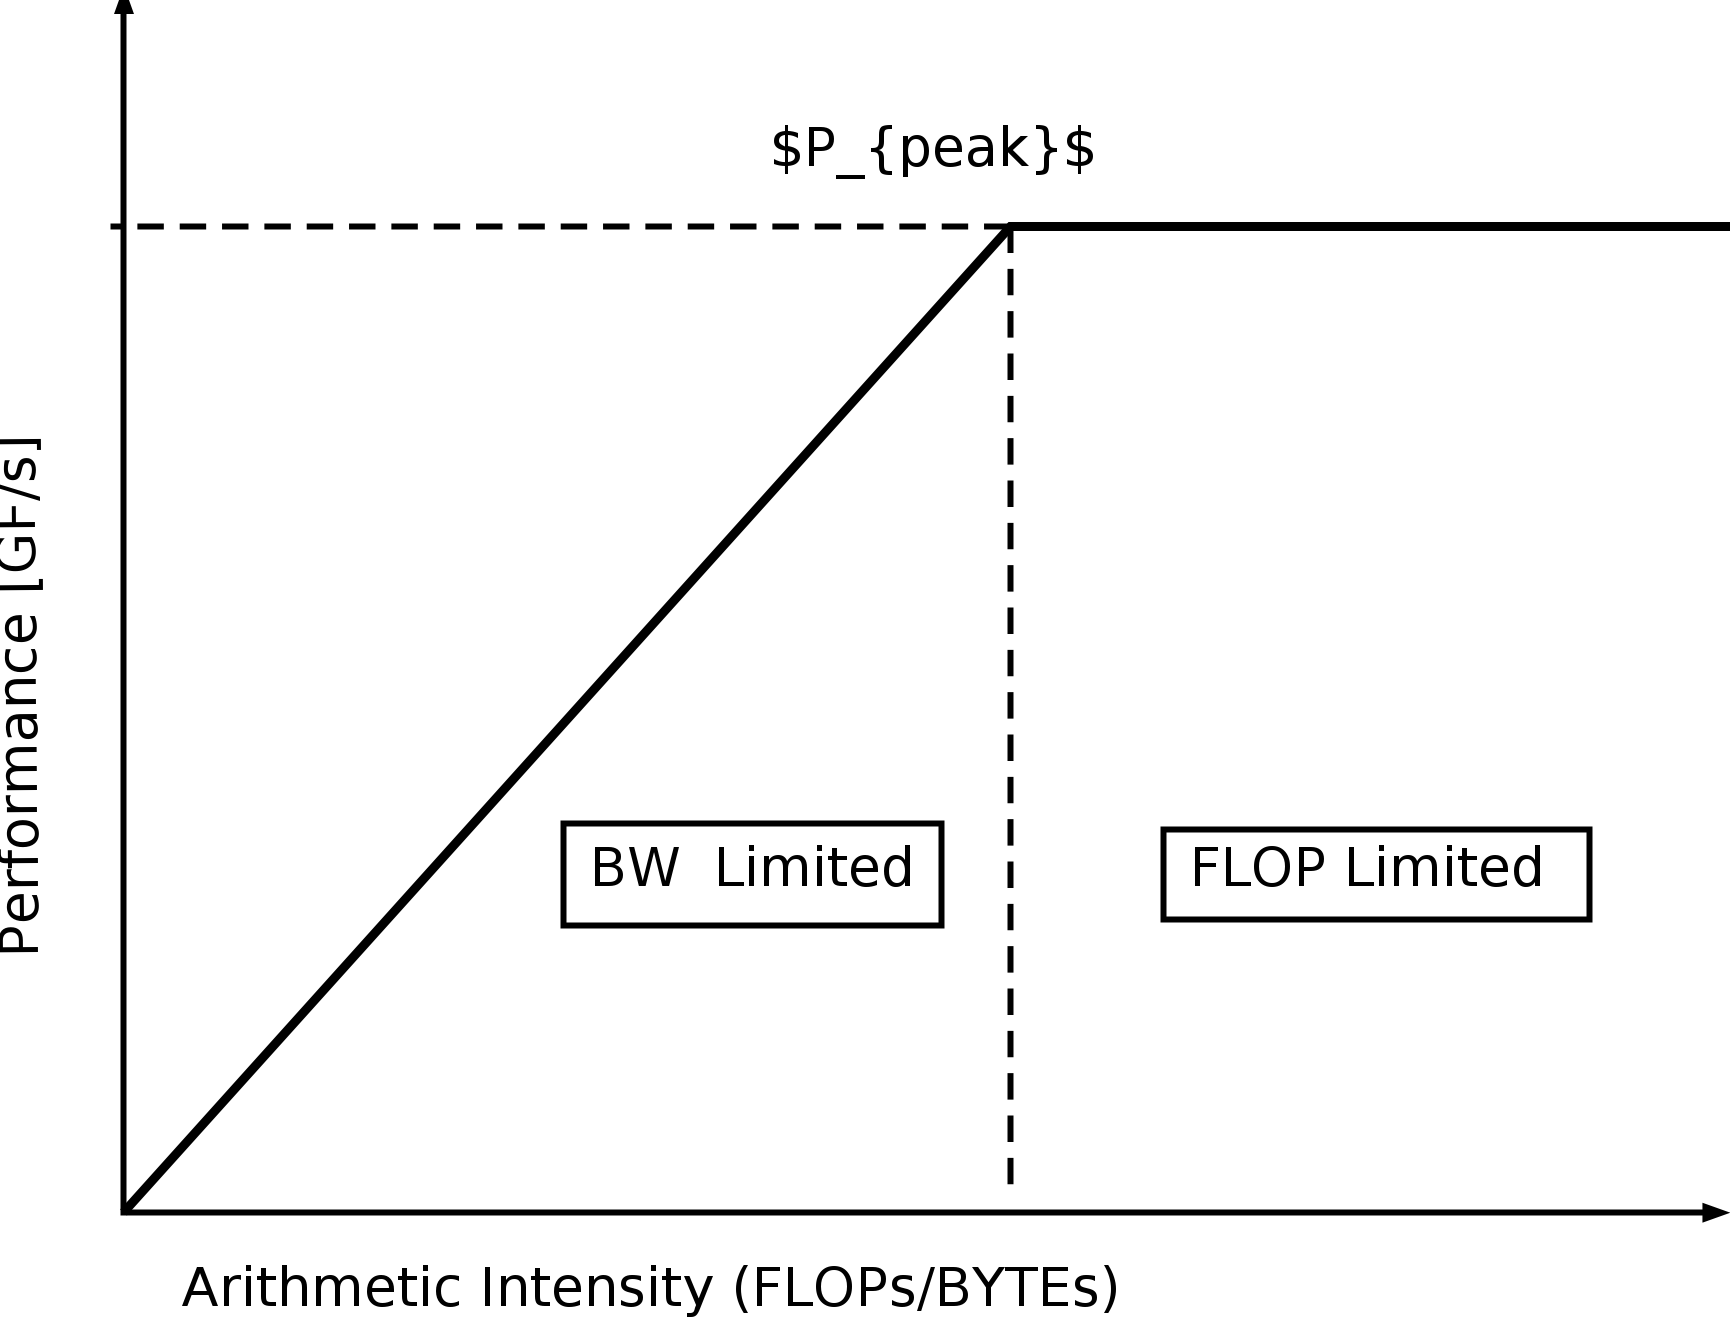
\includegraphics[width=.4\textwidth, height=.3\textwidth]{Roofline_0.png}
    \caption{Roofline Performance Model}
    \label{Roofline_0}
\end{figure}

\begin{equation*}
 GFLOP/s \leq \min \left\{\begin{array}{l}
 Peak \; GFLOP/s \\
 Peak \;GB/s \times Aritmetic \; Intensity
\end{array}\right.
\label{Roofline_eq_2}
\end{equation*}

\begin{table}[!htp]
\centering
\renewcommand{\arraystretch}{2}
\begin{tabular}{|llc|}\hline
Maximum processing capability & Peak performance & $P_{peak} \left[\frac{FLOPs}{s} \right]$ \\ \hline\hline
Rate of revolving door & Memory bandwidth & $b_S\left [\frac{Bytes}{s} \right]$\\ \hline\hline
\multirow{2}{*}{Workload per customer} & \multirow{2}{*}{\begin{tabular}[c]{@{}l@{}}Arithmetic Intensity (AI)\\ or Computational Intensity\end{tabular}} & \multirow{2}{*}{$I \left[\frac{FLOPs}{s} \right]$} \\ 
                       &  & \\ \hline
\end{tabular}
\renewcommand{\arraystretch}{1}
\end{table}

Performance can be estimated from hardware and kernel characteristics
\begin{figure}[!htp]
    \centering
    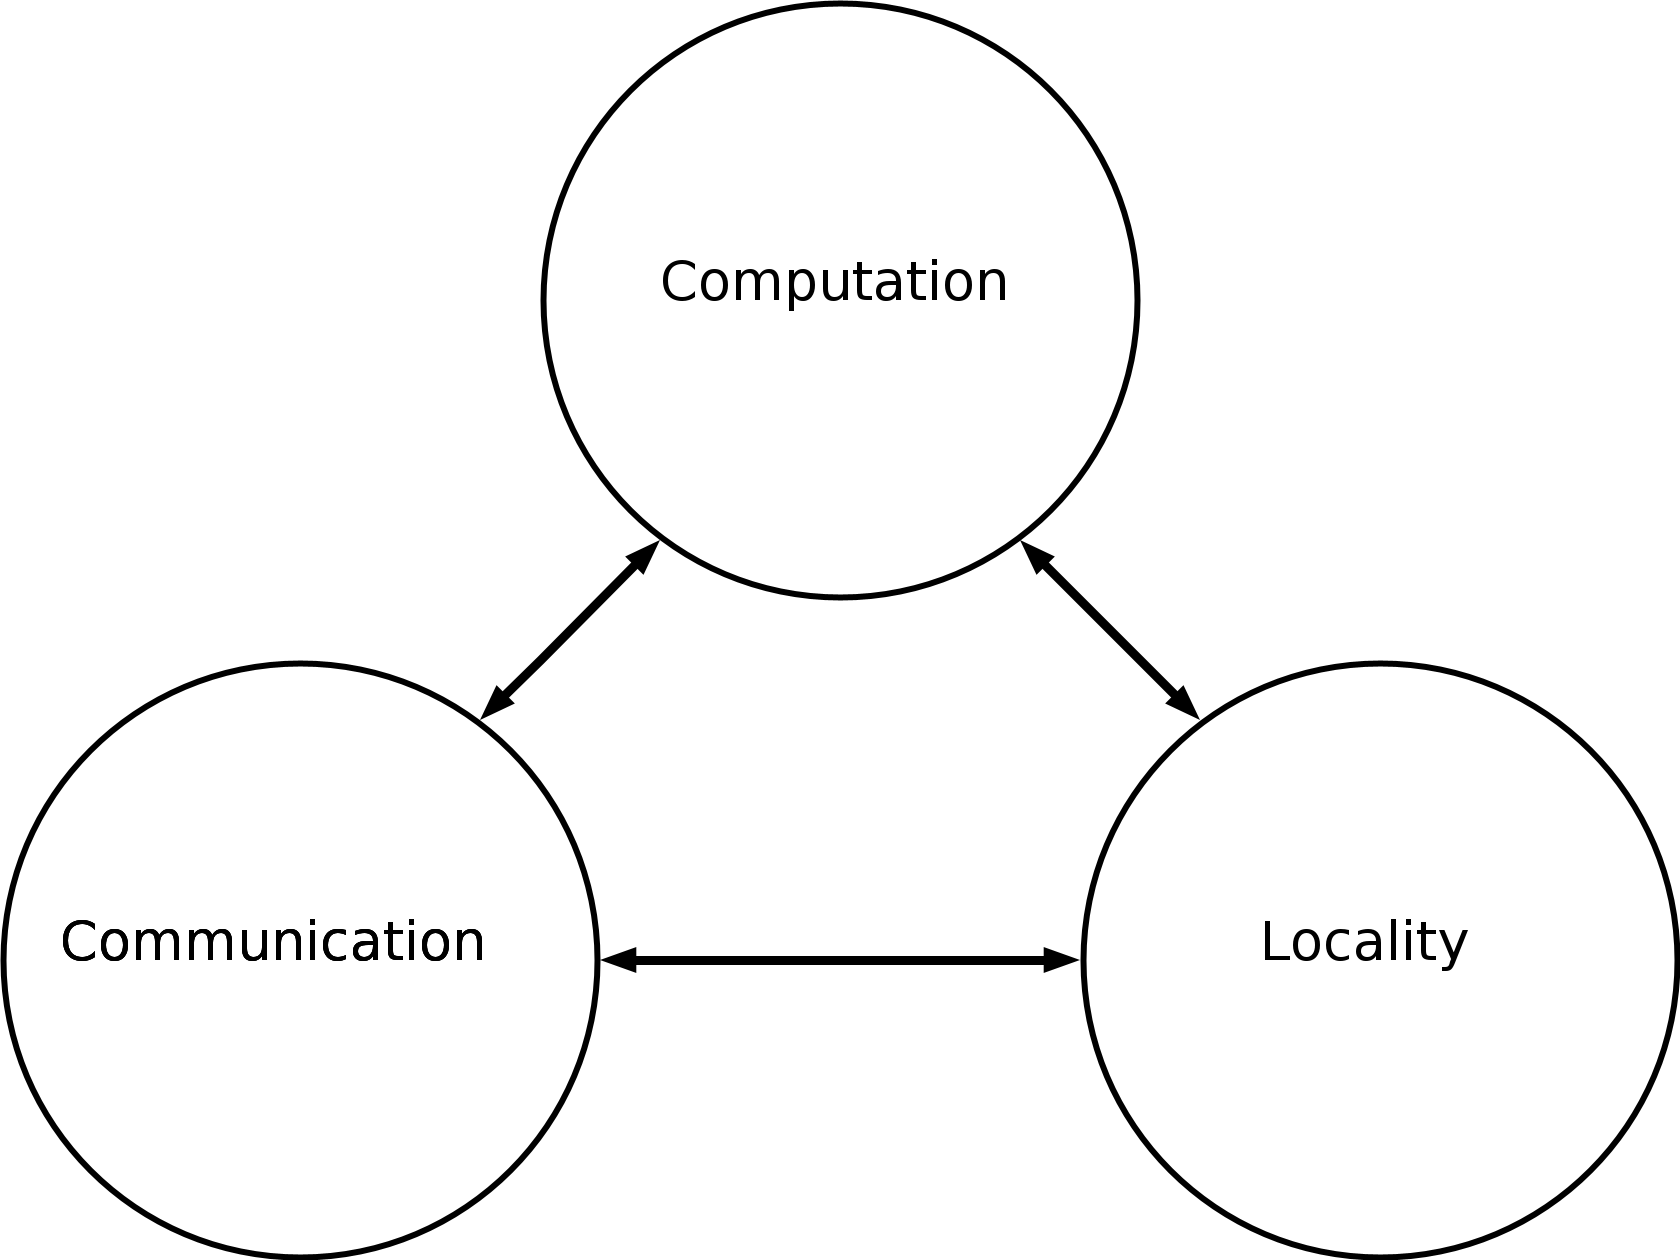
\includegraphics[width=.4\textwidth, height=.3\textwidth]{Roofline_4.png}
    \caption{Roofline model - Principal Components to Performance}
    \label{Roofline_4}
\end{figure}
\begin{itemize}
\item Kernels can be \textbf{compute bounded (DGEMM)} or \textbf{communication bounded (DAXPY)} (kernels are rarely well balanced)
\item Mapping kernel characteristics to hardware characteristics (or vice-versa) lead to performance
\item Some hardware is more 
\begin{itemize}
\item Communication oriented than another (High memory BW)
\item Computation oriented than another (High FLOPs)
\end{itemize}
\item Peak performance
\begin{itemize}
\item High intensity (FLOP Limited): Performance limited by execution
\item Low intensity (BandWidth Limited): Performance limited by bottleneck
\item $P_{max} = I \cdot b_{S}$ (at the red inflexion point)
\end{itemize}
\end{itemize}

\begin{figure}[!htp]
    \centering
    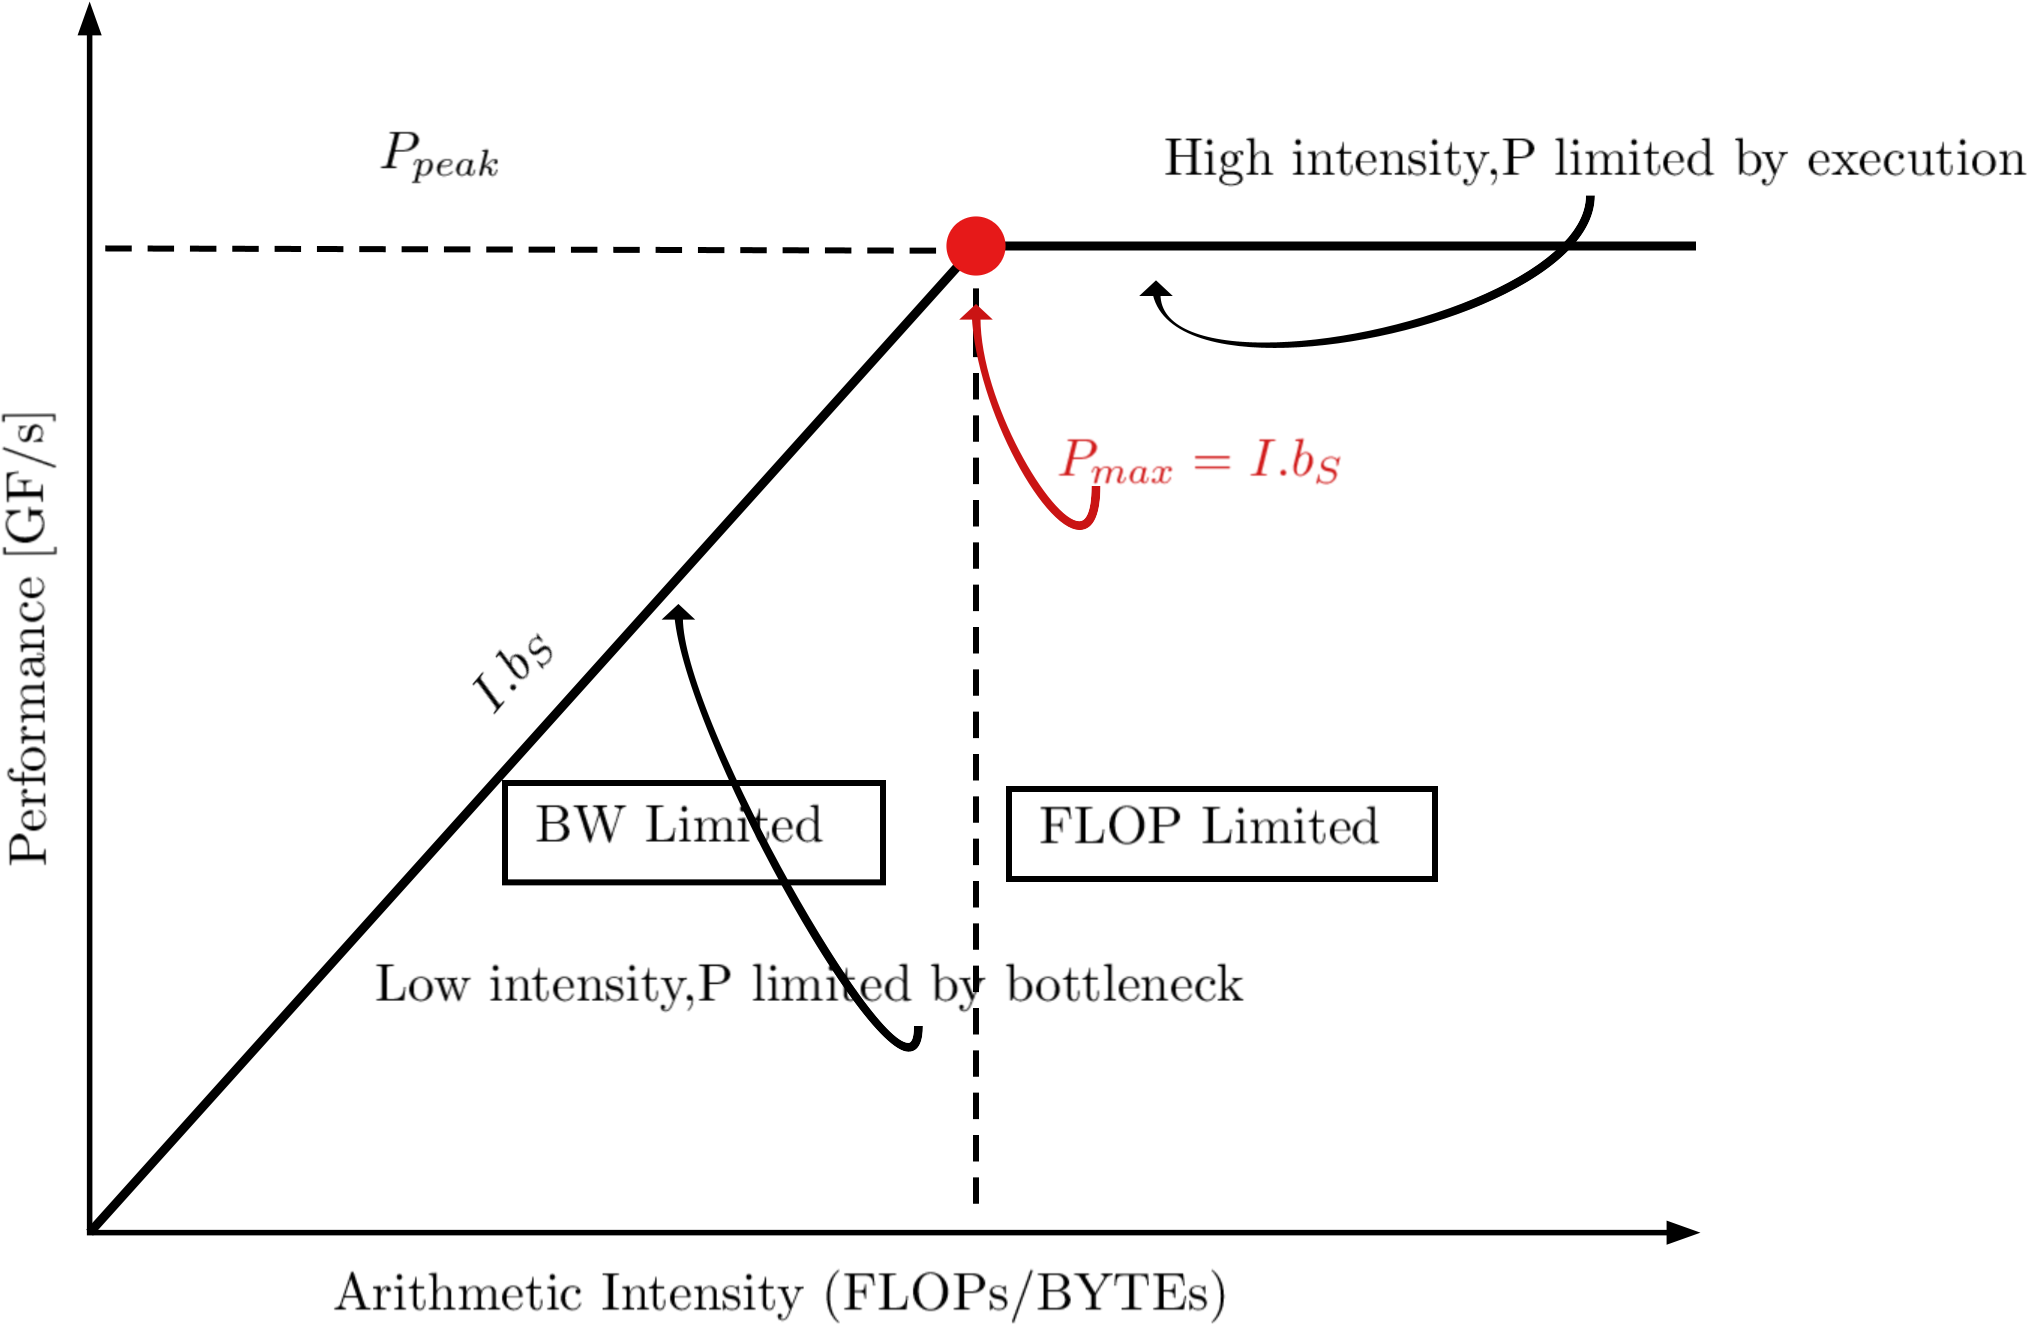
\includegraphics[width=.6\textwidth, height=.4\textwidth]{Roofline_0_1.png}
    \caption{Roofline model - Performance Upper Bounded}
    \label{Roofline_0_1}
\end{figure}
 The Roofline Model – refined
\begin{itemize}
\item $P_{max} = \mbox{Applicable peak performance of a loop}$, assuming that data comes from the level 1 cache (this is not necessarily $P_{peak}$), $P_{max} = 176$ GFlop/s.
\item $I = \mbox{Computational intensity}$ (work per byte transferred) over the slowest data path utilized (code balance $B_C = I^{-1}$ ), $I = 0.167$ Flop/Byte, $B_C = 6$ Byte/Flop.
\item $b_S = \mbox{Applicable (saturated) peak bandwidth}$ of the slowest data path utilized, $b_S = 56$ GByte/s.
\end{itemize}
Expected performance:
\begin{equation*}
 P = \min \left(P_{max} , I \cdot b_S\right) = \min \left(P_{max}, \frac{b_S}{B_C}\right)
\end{equation*}
% [Byte/s]
% [Byte/Flop]

\section{Examples}
\begin{enumerate}
\item Consider DAXPY \\
\begin{minipage}{.35\textwidth} 
\begin{lstlisting}[language=bash,numbers=none,basicstyle=\scriptsize] 
for (i = 0; i < N; ++i) {
   y[i] = a*x[i]+y[i];
}   
\end{lstlisting} 
Execution on BlueGene/Q (Peak 204.8 GFLOP/node).
\end{minipage}
\begin{minipage}{.05\textwidth}
\end{minipage}
\begin{minipage}{.7\textwidth} 
% \begin{figure}[!t]
    \centering
    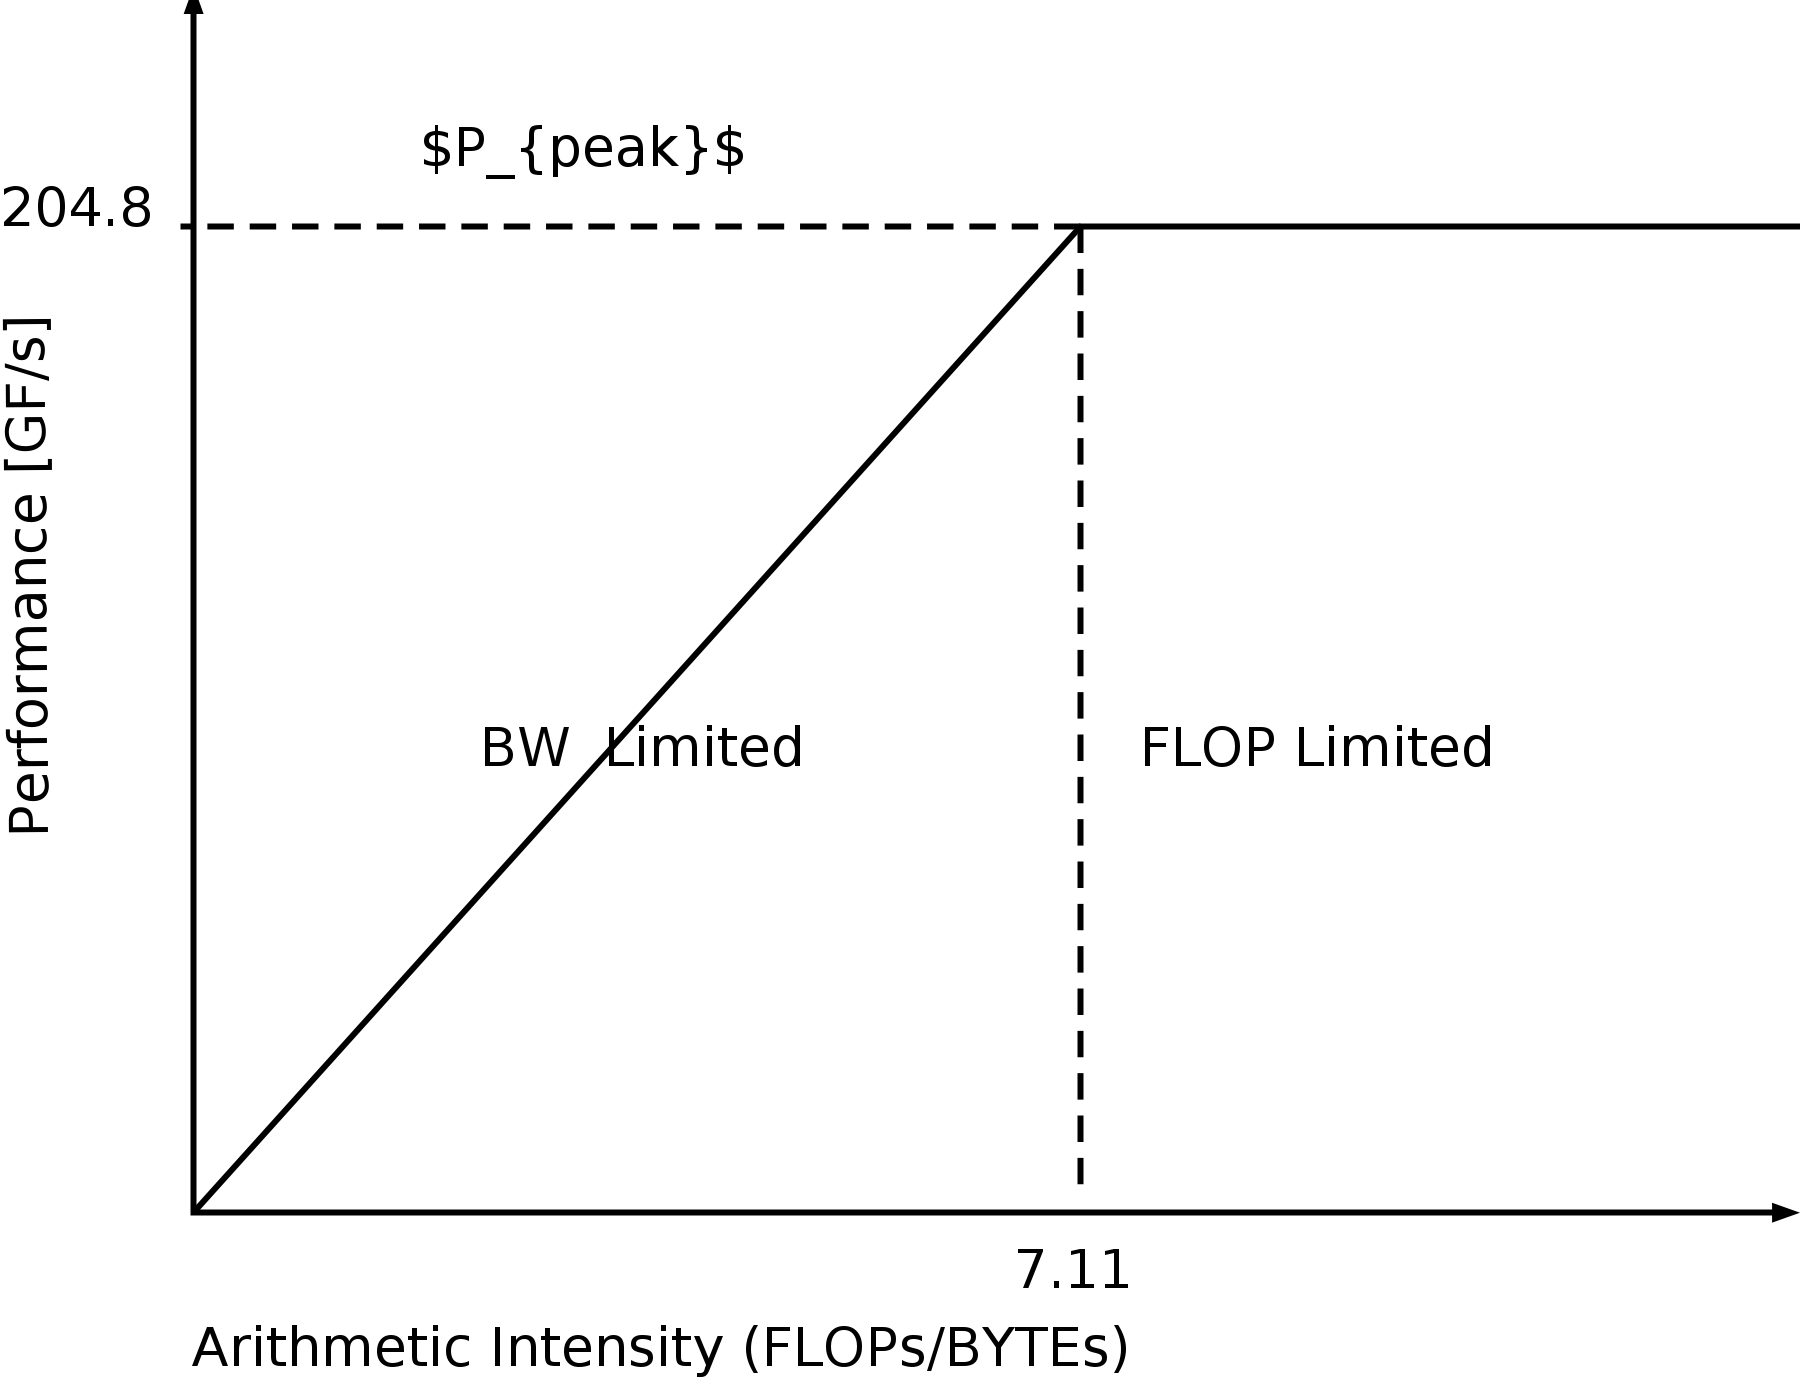
\includegraphics[width=.5\textwidth, height=.4\textwidth]{Roofline_1.png}
    %\caption{Roofline}
    \label{Roofline_1}
% \end{figure}
\end{minipage}
\textbf{Solution :} From the graps, the Peak Performance ($P_{max}$) is \verb+204.8+ GFLOP/s per node, the Aritmetic intensity (AI) is \verb+7.11+ FLOPs/BYTEs, and from the loop the Aritmetic Intensity (AI) can be estimated.
\begin{table}[!htp]
\centering
\begin{tabular}{|l|l|l|l|}
\hline
 LOOPS & FLOPS  & BYTES   & AI $= \frac{FLOPS}{BYTES}$\\\hline\hline
\multirow{3}{*}{\begin{tabular}[c]{@{}l@{}}for (i = 0; i \textless N; ++i)\{ \\ \;\;\;y{[}i{]} = a*x{[}i{]}+y{[}i{]}\\ \}\end{tabular}} &  \multirow{3}{*}{\begin{tabular}[c]{@{}l@{}}1 add\\ 1 mult\end{tabular}}  & \multirow{3}{*}{\begin{tabular}[c]{@{}l@{}}2(8 bytes) loads\\ 1(8 bytes) write (or data transfer)\end{tabular}} & \multirow{3}{*}{$\frac{2}{2*8+1*8}=\frac{1}{12}$} \\
&                        &                                                                                      &       \\
&                        &                                                                                      &       \\\hline
\end{tabular}
\end{table}\\
Then, the loop Peak performance
\[\begin{array}{lcccc}
\mbox{Arithmetic Intensity (AI)}&  & \frac{1}{12} & \longleftrightarrow & 7.11\\
\mbox{Peak performance } (P_{peak})   &  & x            & \longleftrightarrow & 204.8
  \end{array} \]
\begin{minipage}{.35\textwidth} 
The loop AI is in the memory bandwidth (BW) limited area
\begin{equation*}
 x  = \frac{(204.8)\;(1/12)}{(7.11)} = 2.4 \;\frac{GF}{s}
\end{equation*}.
\end{minipage}
\begin{minipage}{.05\textwidth}
\end{minipage}
\begin{minipage}{.7\textwidth} 
% \begin{figure}[!t]
    \centering
    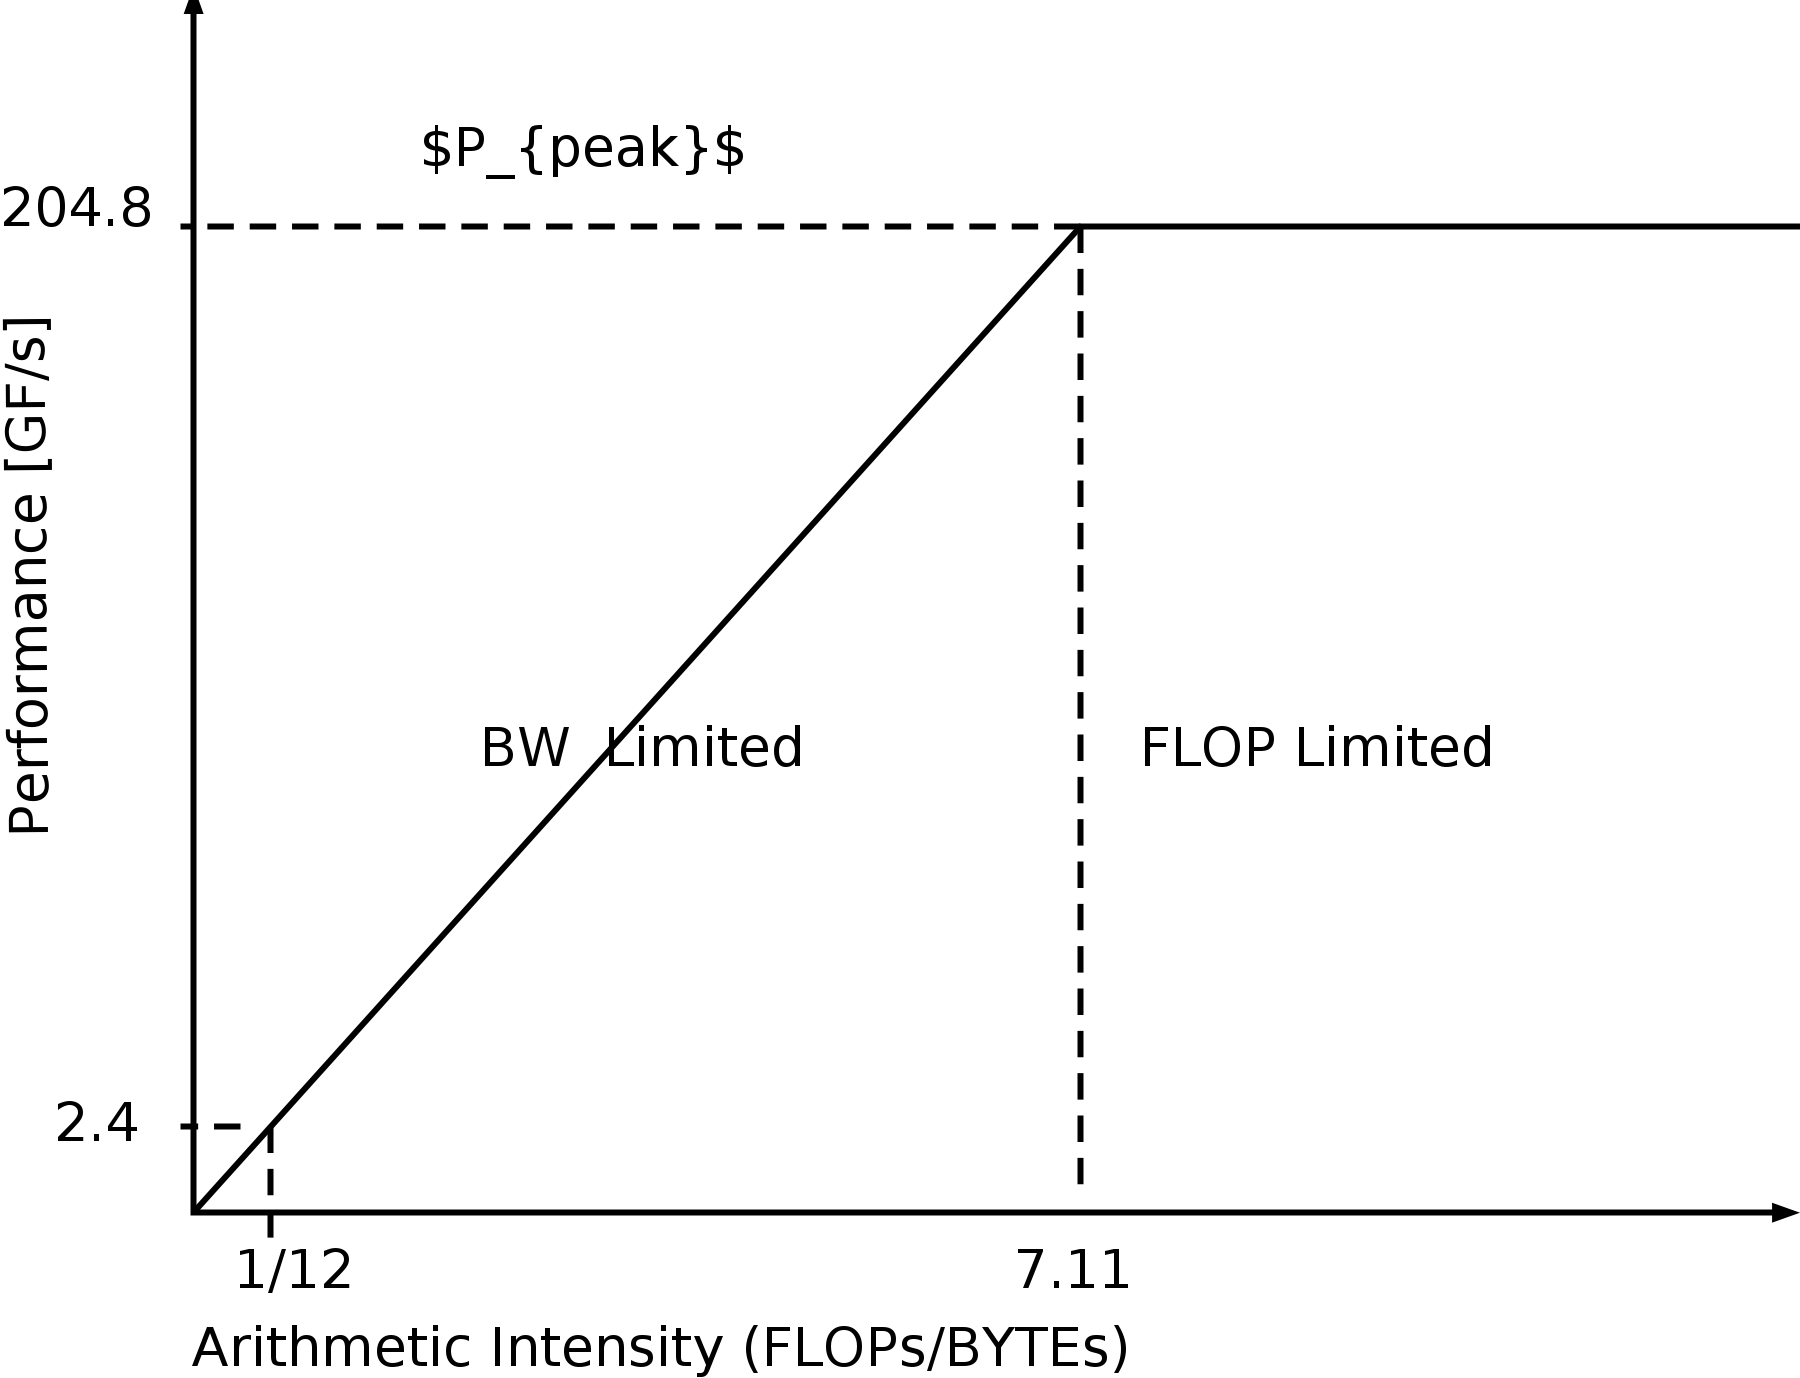
\includegraphics[width=.5\textwidth, height=.4\textwidth]{Roofline_1_2.png}
    %\caption{Roofline}
    \label{Roofline_1}
% \end{figure}
\end{minipage}
\item Consider DAXPY \\
\begin{minipage}{.35\textwidth} 
\begin{lstlisting}[language=bash,numbers=none,basicstyle=\scriptsize] 
for (i = 0; i < N; ++i) {
   y[i] = a*x[i]+y[i]+x[i]*x[i];
}    
\end{lstlisting}  
Execution on BlueGene/Q (Peak 204.8 GFLOP/node).       
\end{minipage}
\begin{minipage}{.05\textwidth}
\end{minipage}
\begin{minipage}{.7\textwidth} 
% \begin{figure}[!t]
    \centering
    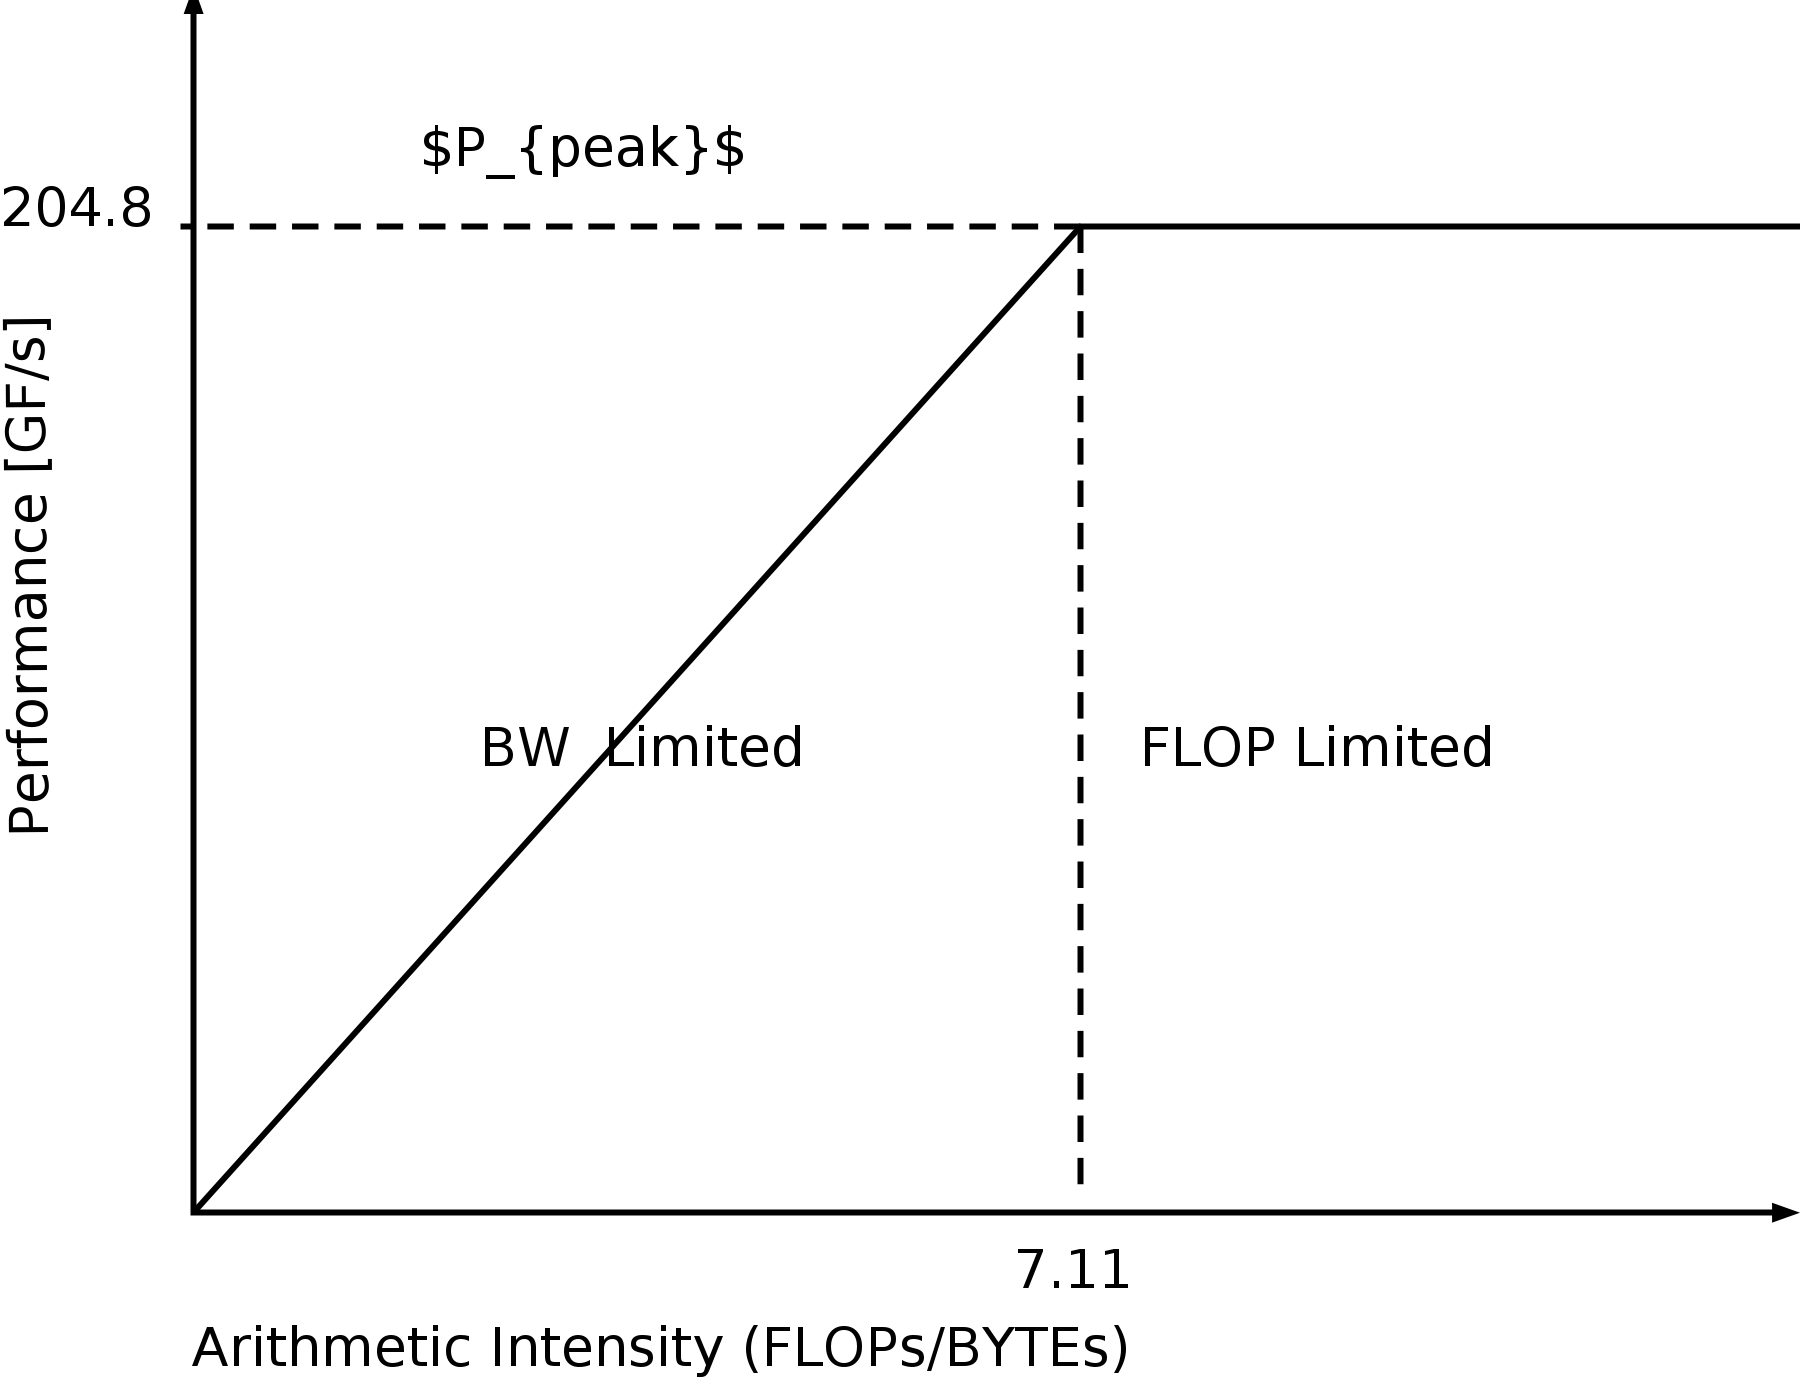
\includegraphics[width=.5\textwidth, height=.4\textwidth]{Roofline_1.png}
    %\caption{Roofline}
    \label{Roofline_1}
% \end{figure}
\end{minipage}
\textbf{Solution :} From the graps, the Peak Performance ($P_{max}$) is \verb+204.8+ GFLOP/s per node, the Aritmetic intensity (AI) is \verb+7.11+ FLOPs/BYTEs, and from the loop the Aritmetic Intensity (AI) can be estimated.
\begin{table}[!htp]
\centering
\begin{tabular}{|l|l|l|l|}
\hline
LOOPS & FLOPS  & BYTES   & AI $= \frac{FLOPS}{BYTES}$\\\hline\hline
\multirow{3}{*}{\begin{tabular}[c]{@{}l@{}}for (i = 0; i \textless N; ++i)\{ \\ \;\;\;y{[}i{]} = a*x{[}i{]}+y{[}i{]}+x{[}i{]}*x{[}i{]}\\ \}\end{tabular}} &  \multirow{3}{*}{\begin{tabular}[c]{@{}l@{}}2 add\\ 2 mult\end{tabular}}  & \multirow{3}{*}{\begin{tabular}[c]{@{}l@{}}2(8 bytes) loads\\ 1(8 bytes) write (or data transfer)\end{tabular}} & \multirow{3}{*}{$\frac{4}{2*8+1*8}=\frac{1}{6}$} \\
&                        &                                                                                      &       \\
&                        &                                                                                      &       \\\hline
\end{tabular}
\end{table}
Performance estimates
\[\begin{array}{lcccc}
\mbox{Arithmetic Intensity}&  & \frac{1}{6} & \longleftrightarrow & 7.11\\
\mbox{Peak performance}    &  & x            & \longleftrightarrow & 204.8
  \end{array} \]
The loop AI is in the memory bandwidth (BW) limited area
\begin{equation*}
 x  = \frac{(204.8)\;(1/6)}{(7.11)} = 4.8 \;\frac{GF}{s}
\end{equation*}

\item Consider two arrays A, and B, both have dimension of $N\times N$\\
\begin{minipage}{.4\textwidth} 
\begin{lstlisting}[language=bash,numbers=none,basicstyle=\scriptsize] 
for (i = 0; i < N; ++i) {
    for (j = 0; j < N; ++j) {
        B[i][j] = A[i-2][j] + A[i-1][j] + C*A[i][j] +
                  A[i+1][j] + A[i+2][j] + A[i][j-2] + 
                  A[i][j-1] + A[i][j+1] + A[i][j+2];
}    
\end{lstlisting}   
Execution on BlueGene/Q (Peak 204.8 GFLOP/node).
\end{minipage}
\begin{minipage}{.6\textwidth} 
% \begin{figure}[!t]
    \centering
    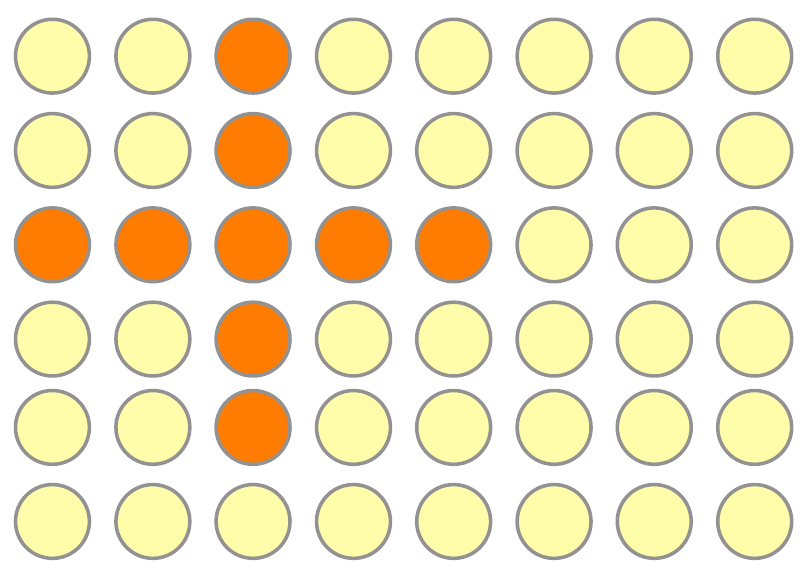
\includegraphics[width=.5\textwidth, height=.5\textwidth]{2D_array.png}
    %\caption{Roofline}
    \label{2D_array}
% \end{figure}
\end{minipage}
\textbf{Solution :} From the graps, the Peak Performance ($P_{max}$) is \verb+204.8+ GFLOP/s per node, the Aritmetic intensity (AI) is \verb+7.11+ FLOPs/BYTEs, and from the loop the Aritmetic Intensity (AI) can be estimated.
\begin{table}[!htp]
\centering
\begin{tabular}{|l|l|l|l|}
\hline
LOOPS & FLOPS  & BYTES   & AI $= \frac{FLOPS}{BYTES}$\\\hline\hline
\multirow{3}{*}{\begin{tabular}[c]{@{}l@{}}for (i = 0; i \textless N; ++i)\{ \\
\;\; for (j = 0; j \textless N; ++j)\{\\ \;\;\;\;\;B{[}i{]}{[}j{]} = A{[}i-2{]}{[}j{]}+A{[}i-1{]}{[}j{]}+A{[}i{]}{[}j{]}\\ 
\;\;\;\;\;\;\;\;\;\;A{[}i+1{]}{[}j{]}+A{[}i+2{]}{[}j{]}+A{[}i{]}{[}j-2{]}\\ 
\;\;\;\;\;\;\;\;\;\;A{[}i{]}{[}j-1{]}+A{[}i{]}{[}j+1{]}+A{[}i{]}{[}j+2{]}\\ 
\}\end{tabular}} &  \multirow{3}{*}{\begin{tabular}[c]{@{}l@{}}8 add\\ 1 mult\end{tabular}}  & \multirow{3}{*}{\begin{tabular}[c]{@{}l@{}}1(8 bytes) loads\\ 1(8 bytes) write (or data transfer)\end{tabular}} & \multirow{3}{*}{$\frac{9}{1*8+1*8}=\frac{1}{2}$} \\
&                        &                                                                                      &       \\
&                        &                                                                                      &       \\
&                        &                                                                                      &       \\
&                        &                                                                                      &       \\
&                        &                                                                                      &       \\\hline
\end{tabular}
\end{table}\\
Performance estimates
\[\begin{array}{lcccc}
\mbox{Arithmetic Intensity}&  & \frac{1}{2} & \longleftrightarrow & 7.11\\
\mbox{Peak performance}    &  & x            & \longleftrightarrow & 204.8
  \end{array} \]
The loop AI is in the memory bandwidth (BW) limited area
\begin{equation*}
 x  = \frac{(204.8)\;(1/2)}{(7.11)} = 14.4 \;\frac{GF}{s}
\end{equation*}
\item Apply this example to performance of compute devices\\
\begin{table}[!htp]
\centering
\begin{tabular}{|l|l|l|l|}
\hline
 LOOPS & FLOPS  & BYTES   & AI $= \frac{FLOPS}{BYTES}$\\\hline\hline
\multirow{3}{*}{\begin{tabular}[c]{@{}l@{}} double s = 0; \\ double a[];\\ for (i = 0; i \textless N; ++i)\{ \\ \;\;\;s = s + a{[}i{]}* a{[}i{]}\\ \}\end{tabular}} &  \multirow{3}{*}{\begin{tabular}[c]{@{}l@{}}1 add\\ 1 mult\end{tabular}}  & \multirow{3}{*}{\begin{tabular}[c]{@{}l@{}}1(8 bytes) loads\end{tabular}} & \multirow{3}{*}{$\frac{2}{1*8}=\frac{2}{8}$} \\
&                        &                                                                                      &       \\
&                        &                                                                                      &       \\
&                        &                                                                                      &       \\
&                        &                                                                                      &       \\\hline
\end{tabular}
\end{table}
\begin{minipage}{.3\textwidth} 
\begin{lstlisting}[language=bash,numbers=none,basicstyle=\scriptsize] 
double s = 0; 
double a[];
for (i = 0; i < N; ++i) {
    s = s + a[i] * a[i];
}    
\end{lstlisting} 
\begin{eqnarray*}
P_{peak}  &  = & 4 \frac{GFLOPs}{s}\\
b_S & = & 10 \frac{GBytes}{s}
\end{eqnarray*}
\end{minipage}
\begin{minipage}{.1\textwidth} 
\end{minipage}
\begin{minipage}{.6\textwidth} 
% \begin{figure}[!htp]
    \centering
    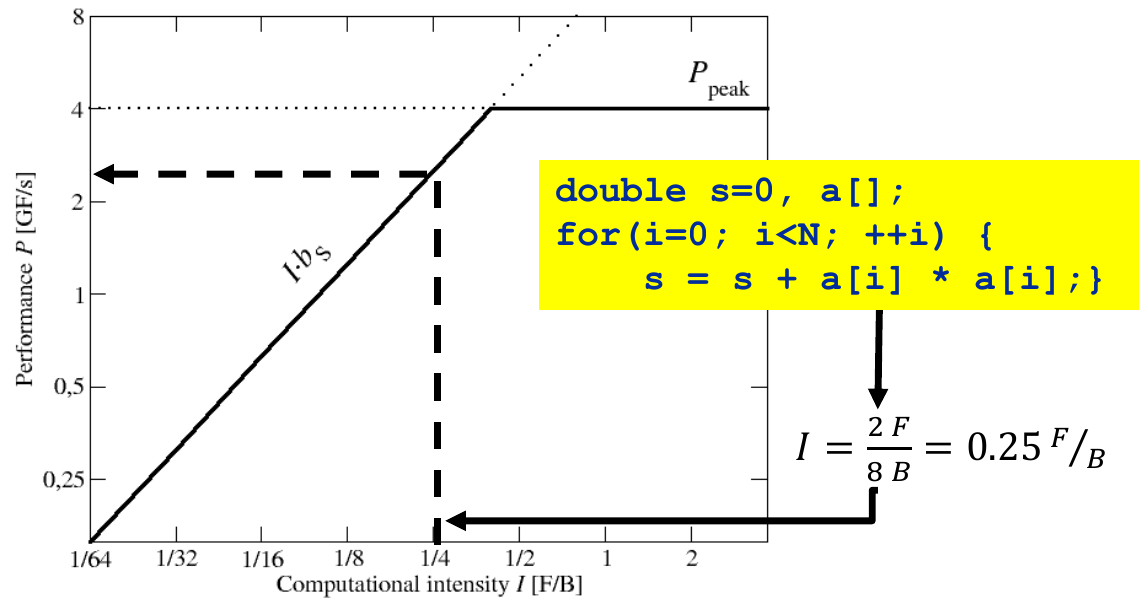
\includegraphics[width=1\textwidth, height=.6\textwidth]{Roofline_3.png}
%    \caption{Roofline}
%     \label{Roofline_1}
% \end{figure}
\end{minipage}
\item Estimate $P_{max}$ of vector triad on Haswell\\
\begin{table}[!htp]
\centering
\begin{tabular}{|l|l|l|l|}
\hline
 LOOPS & FLOPS  & BYTES   & AI $= \frac{FLOPS}{BYTES}$\\\hline\hline
\multirow{3}{*}{\begin{tabular}[c]{@{}l@{}} double $^{*}A,\; ^{*}B,\; ^{*}C,\; ^{*}D$;\\ for (i = 0; i \textless N; ++i)\{ \\ \;\;\;A{[}i{]} = B{[}i{]} + C{[}i{]} * D{[}i{]}\\ \}\end{tabular}} &  \multirow{3}{*}{\begin{tabular}[c]{@{}l@{}}1 add\\ 1 mult\end{tabular}}  & \multirow{3}{*}{\begin{tabular}[c]{@{}l@{}}3(8 bytes) loads\\1(8 bytes) write (or data transfer) \end{tabular}} & \multirow{3}{*}{$\frac{2}{3*8+1*8}=\frac{2}{32}$} \\
&                        &                                                                                      &       \\
&                        &                                                                                      &       \\
&                        &                                                                                      &       \\
&                        &                                                                                      &       \\\hline
\end{tabular}
\end{table}
\begin{minipage}{.3\textwidth} 
\begin{lstlisting}[language=bash,numbers=none,basicstyle=\scriptsize] 
double *A, *B, *C, *D;
for (int i=0; i<N; i++) {
 A[i] = B[i] + C[i] * D[i];
}
\end{lstlisting} 
\begin{eqnarray*}
P_{peak}  &  = & 4 \frac{GFLOPs}{s}\\
b_S & = & 10 \frac{GBytes}{s}
\end{eqnarray*}
\end{minipage}
\begin{minipage}{.1\textwidth} 
\end{minipage}
\begin{minipage}{.6\textwidth} 
% \begin{figure}[!htp]
%     \centering
%     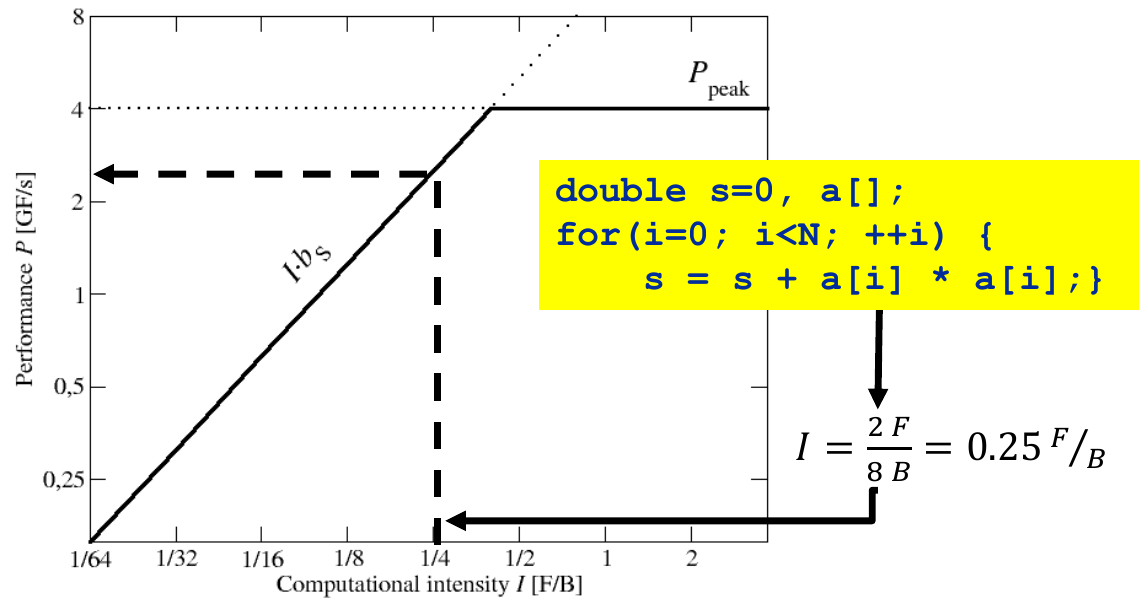
\includegraphics[width=1\textwidth, height=.6\textwidth]{Roofline_3.png}
%    \caption{Roofline}
%     \label{Roofline_1}
% \end{figure}
\end{minipage}


Minimum number of cycles to process one AVX-vectorized iteration (one core)? 

Equivalent to 4 scalar iterations
\begin{description}
 \item [Cycle 1:] \textbf{LOAD + LOAD + STORE}
 \item [Cycle 2:] LOAD + LOAD + \textbf{FMA} + FMA
 \item [Cycle 3:] LOAD + LOAD + STORE
 \item [Answer:] 1.5 cycles
\end{description}

What is the performance in GFlops/s per core and the bandwidth in GBytes/s? \\

One AVX iteration (1.5 cycles) does $4 \times 2 = 8$ flops:
\begin{equation*}
\frac{2.3 \times 10^9 \; cy/s}{1.5 \; cy}\times 4\; updates\; \frac{2 \; flops}{update} = 12.27 \; \frac{Gflops}{s}
\end{equation*}

\begin{equation*}
 6.13 \times 10^9 \; \frac{updates}{s} \times 32 \;\frac{bytes}{update} = 196 \; \frac{Gbyte}{s}
\end{equation*}

Vector triad $A(:)=B(:)+C(:)*D(:)$ on a 2.3 GHz 14-core Haswell chip (AVX vectorized)
\begin{itemize}
\item Peak memory bandwidth: $b_S = 50 \; \frac{GB}{s}$
\item Memory code balance:
\begin{itemize}
\item $B_c = \frac{(4+1) \; Words}{2 \; Flops} = 20 \; \frac{B}{F}$ (including write allocate)
\item $I = 0.05 \; \frac{F}{B}$
\item $I \cdot b_S = 0.05 \; \frac{F}{B} \times 50 \; \frac{GB}{s} = 2.5 \; \frac{GF}{s}$ (0.5\% of peak performance)
\end{itemize}
\end{itemize}


\begin{itemize}
 \item $P_{peak} = 515.2 \; \frac{Gflop}{s} \; (14 \;cores \times (8+8) \frac{Flops}{cy} \times 2.3 \;GHz)$
\item $P_{max} = 14 \times 12.27 \; \frac{Gflop}{s} = 172\; \frac{Gflop}{s}$ (33\% peak)
\end{itemize}

\begin{equation}
P= \min \left(P_{max}, I \cdot b_S\right) = \min \left(172,2.5\right) \; GFlop/s = 2.5 \; GFlop/s
\end{equation}



\item  NVIDIA’s latest V100 GPU : 
\begin{itemize}
 \item Each GV100 Streaming Multiprocessor (SM) consists of four processing blocks (warp schedulers)
 \item Each warp scheduler can dispatch one instruction per cycle. 
\end{itemize}
As such, the theoretical maximum (warp-based) \verb+instruction/s+ is
\begin{equation}
 80(\mbox{SM}) \times 4(\mbox{warp scheduler}) times 1(\mbox{instruction/cycle}) \times 1.53(\mbox{GHz}) = 489.6 GIPS
\end{equation}
\begin{itemize}
\item Memory access is coalesced into transactions. 
\begin{itemize}
\item The transaction size for global/local memory, the L2 cache, and HBM are 32 bytes. 
\item The shared memory transaction size is 128 bytes. 
\item In practice, a warp-level load may generate anywhere from 1 to 32 transactions depending on memory patterns. 
\end{itemize}
\item This makes the transaction the natural unit when analyzing memory access. 
\item We leverage Yang et al.’s methodology for measuring GPU bandwidths but rescale into billions of transactions per second (GTXN/s) based on the transaction size.
\end{itemize}
shows the resultant Instruction Roofline ceilings for the GV100. L1, L2, and HBM bandwidths of 14000, 2996, and 828 GB/s sustain 437, 93.6, and 25.9 GTXN/s when normalized to
the typical 32-byte transaction size.
\begin{equation}
 GIPS \leq \min \left\{\begin{array}{l}
 Peak \; GIPS \\
 Peak \;GT\times N/s \times Instruction\; Intensity
\end{array}\right.
\label{Roofline_eq_1}
\end{equation}

\item (NERSC-Cori Haswell/KNL) Xeon Phi 7250 (HLRN Cray TDS), advertised with 3.05 TFLOPS peak DP (peak double precision performance).% https://docs.nersc.gov/systems/cori/
% https://www.nersc.gov/about/nersc-history/history-of-systems/
Intel Xeon Phi Processor 7250 68C 
\begin{itemize}
 \item Processor speed (Clock rate) : 1.4GHz
 \item Architecture    : x86-64
 \item Physical Cores Per Node :  68
 \item Theoretical peak : 3 TFlops/node
 \item 8 SIMD (Single Instruction/Multiple Data)
 \item 2 FMS (Fused Multiply-Add instructions) is an extension to the 128 and 256-bit Streaming SIMD Extensions instructions in the x86 microprocessor instruction set to perform fused multiply–add (FMA) operations.
 \item VPUs : Vector processing units (VPUs) perform the actual work of computing a SIMD vector operation in parallel. 
\end{itemize}



\begin{lstlisting}[language=bash,numbers=none,basicstyle=\tiny]
1.4 GHz x 68 core x 8 SIMD x 2 VPUs x 2 FMA = 3046.4 GFLOPS
\end{lstlisting}

\begin{lstlisting}[language=bash,numbers=none,basicstyle=\tiny]
AVX frequency is only 1.2 GHz and might throttle down under heavy load => actual peak: 2611.2 GFLOPS
\end{lstlisting}
\end{enumerate}






% \begin{itemize}
% \item Open a terminal \verb!CTRL + ALT + T!
% \item Remember, login with \verb+wtrw.land.gov+ (\verb+front-end+ ) and next login with \verb+gr-fe+ or \verb+ba-fe+ (\verb+back-end+)
% \item Login into 
% \end{itemize}
% \begin{lstlisting}[language=bash,numbers=none,basicstyle=\tiny] 
% hrmoncada:Memory_leak_#350$ git clone https://github.com/pwolfram/MPAS-Model.git ocean_tracer
% Cloning into 'MPAS-Model'...
% remote: Enumerating objects: 136, done.
% remote: Counting objects: 80% (136/136), done.
% remote: Compressing objects: 80% (86/86), done.
% remote: Total 46698 (delta 79), reused 98 (delta 50), pack-reused 46562
% Receiving objects: 80% (46698/46698), 18.78 MiB | 6.79 MiB/s, done.
% Resolving deltas: 80% (36026/36026), done.
% Checking connectivity... done.
% \end{lstlisting}
% 
% \begin{lstlisting}[language=bash,numbers=none,basicstyle=\scriptsize,linebackgroundcolor={%
%     \ifnum\value{lstnumber}=6 \color{green!60} \fi
%     \ifnum\value{lstnumber}=8 \color{yellow!70} \fi
%     \ifnum\value{lstnumber}=8 \color{blue!45} \fi  
%     \ifnum\value{lstnumber}=11 \color{gray!80} \fi
%     \ifnum\value{lstnumber}=14 \color{red!50} \fi
%     }]
% gr-fe1:MPAS-O_V6.0_RRS30to8$ ll
% total 5935993
% -rw-r----- 1 hrmoncada hrmoncada   93551680 Nov 27  2017 forcing_data.nc
% -rw-r----- 1 hrmoncada hrmoncada   63714293 Nov 27  2017 graph.info
% -rw-r----- 1 hrmoncada hrmoncada    5450056 Nov 27  2017 graph.info.part.480
% lrwxrwxrwx 1 hrmoncada hrmoncada         97 Mar  7 17:02 metis -> /turquoise/usr/projects/climate/mpeterse/software/metis-5.1.0/build/Linux-x86_64/programs/gpmetis
% -rw-r----- 1 hrmoncada hrmoncada      31242 May 22  2018 namelist.ocean
% lrwxrwxrwx 1 hrmoncada hrmoncada         60 Mar  7 17:02 ocean_model -> /usr/projects/climate/hrmoncada/repos/MPAS-Model/ocean_model
% -rw-r----- 1 hrmoncada hrmoncada 9304573052 May 22  2018 oRRS30to8v3.171128.nc
% lrwxrwxrwx 1 hrmoncada hrmoncada         94 Mar  7 17:03 performance_test.py -> /usr/projects/climate/hrmoncada/repos/MPAS-Tools/ocean/performance_testing/performance_test.py
% lrwxrwxrwx 1 hrmoncada hrmoncada         93 Mar  7 17:02 plot_from_files.py -> /usr/projects/climate/hrmoncada/repos/MPAS-Tools/ocean/performance_testing/plot_from_files.py
% -rwxr-x--- 1 hrmoncada hrmoncada        
% \subsection{login into }
% \begin{itemize}
% \item Open a terminal \verb!CTRL + ALT + T!
% \item Remember, login with \verb+wtrw.land.gov+ (\verb+front-end+ ) and next login with \verb+gr-fe+ or \verb+ba-fe+ (\verb+back-end+)
% \item Login into 
% \begin{itemize}
% \item \verb+badger+ 
% \begin{lstlisting}[language=bash,numbers=none] 
% $ ba
% hrmoncada@wtrw.lanl.gov's password:     <== front-end
% .
% ba-fe1:~$                               <== back-end  
% \end{lstlisting}


% \begin{itemize}
% \item 
% \begin{lstlisting}[language=bash,numbers=none] 
% 
% \end{lstlisting}
%  \item 
% \begin{lstlisting}[language=bash,numbers=none] 
% 
% \end{lstlisting}
% \end{itemize}
% \item 
% \begin{lstlisting}[language=bash,numbers=none] 
% 
% \end{lstlisting}
% \begin{lstlisting}[language=bash,numbers=none] 
% 
% \end{lstlisting}
% \end{itemize}

% \subsection{Trasfer your test cases into IC}
% \begin{itemize}
% \item Download test cases from
% % \begin{lstlisting}[language=bash,numbers=none] 
% % 
% % \end{lstlisting}
% \begin{figure}[htp!]
%     \centering
%     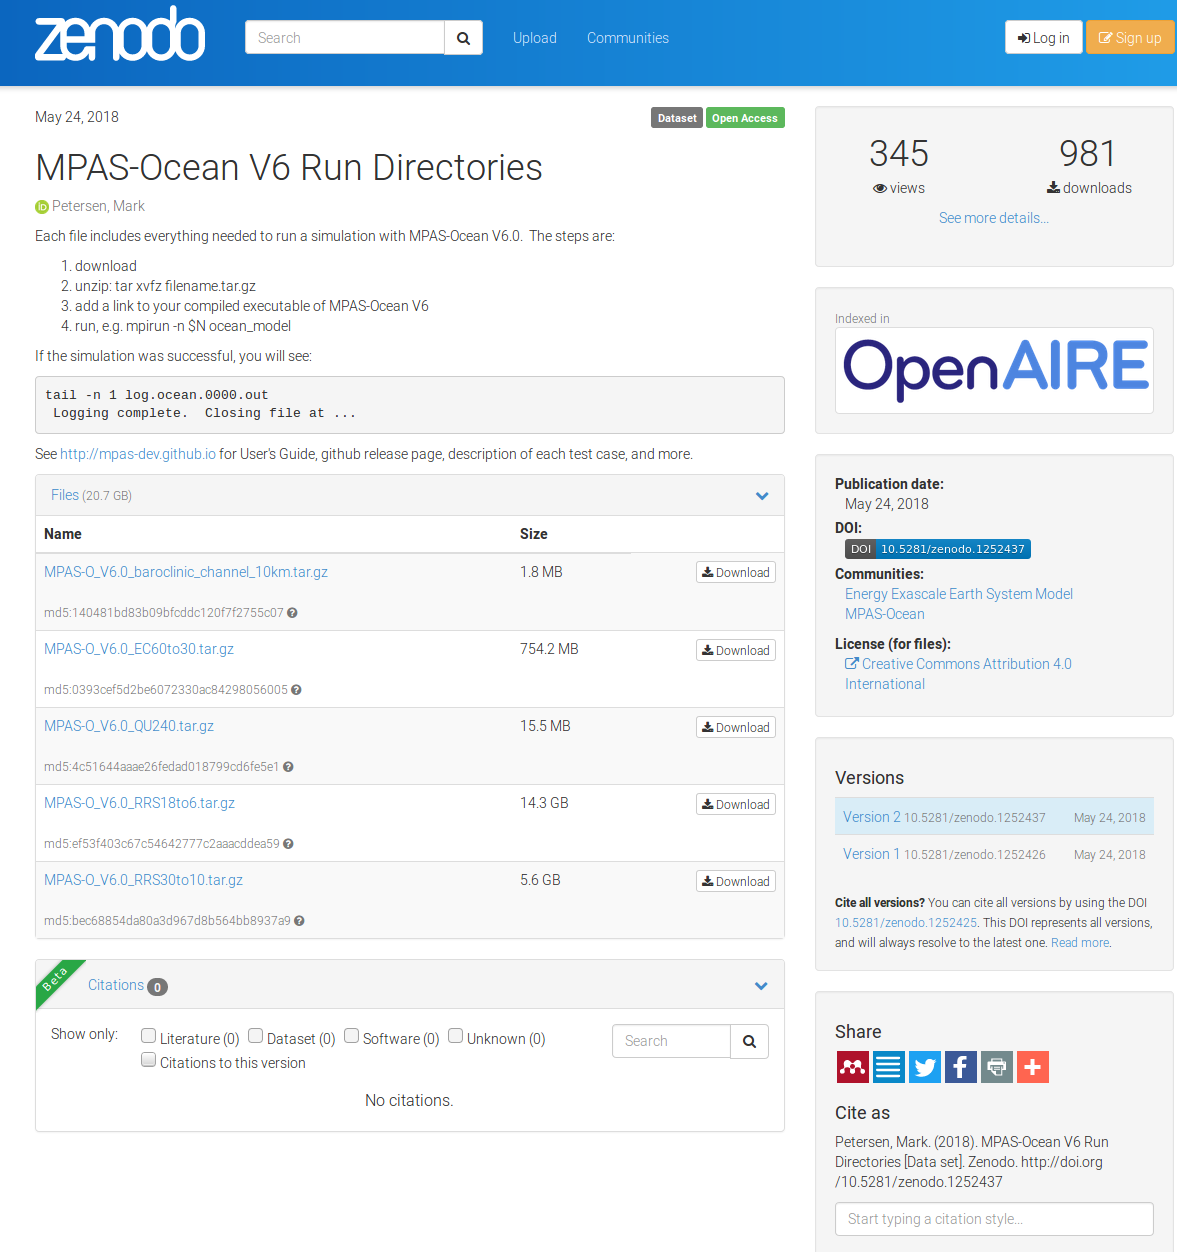
\includegraphics[width=.7\textwidth, height=.6\textwidth]{Zenodo_test_cases.png}
%     \caption{Zenodo Test Cases}
%     \label{Zenodo_test_cases.png}
% \end{figure}
% \item Trasfer the files from your Desktop to your \verb+scratch+ workspace
% \begin{lstlisting}[language=bash,numbers=none] 
% 
% \end{lstlisting}
% \item Tranfer test files into \verb+Zenodo_Scratch+ folder 
% \begin{lstlisting}[language=bash,numbers=none,basicstyle=\scriptsize] 
%             
% \end{lstlisting}
% \end{itemize}
% 
% \begin{enumerate}
% \item Submit job
% \begin{lstlisting}[language=bash,numbers=none,basicstyle=\scriptsize] 
% 
% \end{lstlisting}
% \begin{lstlisting}[language=bash,numbers=none,basicstyle=\scriptsize] 
% 
% \end{lstlisting}

% \item Navegate into the \verb+figure_performance+ folder
% \begin{lstlisting}[language=bash,numbers=none] 
% gr-fe1:MPAS-O_V6.0_RRS30to8$ cd figures_performance/
% gr-fe1:figures_performance$ ll
% total 80
% -rw-rw---- 1 hrmoncada hrmoncada 3806 Mar  7 18:00 RRS30to8_grizzly_824_20190307_175036.png
% \end{lstlisting}
% \item Display figure (see Figure \ref{RRS30to8_grizzly_824_20190307_175036.png})
% \begin{lstlisting}[language=bash,numbers=none] 
% ba-fe1:figures_performance$ display  RRS30to8_grizzly_824_20190307_175036.png
% \end{lstlisting}
% \begin{figure}[htp!]
%     \centering
%     \includegraphics[width=1\textwidth, height=.4\textwidth]{RRS30to8_grizzly_824_20190307_175036.png}
%     \caption{MPAS-O\_V6.0\_baroclinic\_channel\_8km}
%     \label{RRS30to8_grizzly_824_20190307_175036.png}
% \end{figure}
% \end{enumerate}


% \item On \verb+/lustre/scratch3/turquoise/mpeterse/runs/MPAS-O_V6.0/MPAS-O_V6.0_QU240+
% \begin{lstlisting}[language=bash,numbers=none,linebackgroundcolor={%
%     \ifnum\value{lstnumber}=1 \color{green!35} \fi
%     \ifnum\value{lstnumber}=3 \color{green!35} \fi
%     \ifnum\value{lstnumber}=5 \color{green!35} \fi 
%     \ifnum\value{lstnumber}=7 \color{green!35} \fi
%     \ifnum\value{lstnumber}=9 \color{green!35} \fi }]
% lrwxrwxrwx  1 mpeterse mpeterse   97 Jun 12  2018 metis -> 
% /turquoise/usr/projects/climate/mpeterse/software/metis-5.1.0/build/Linux-x86_64/programs/gpmetis
% lrwxrwxrwx  1 mpeterse mpeterse   82 Sep 8 13:58 ocean_model -> 
% /usr/projects/climate/mpeterse/repos/model/ocean_develop/ocean_model_18098_0b984bd_gr_gfortran_openmp
% lrwxrwxrwx  1 mpeterse mpeterse   120 Sep 8 13:57 performance_test.py -> 
% /usr/projects/climate/mpeterse/repos/tools/divya_ocean_performance_testing/ocean/performance_testing/performance_test.py
% lrwxrwxrwx  1 mpeterse mpeterse   119 Sep 8 13:57 plot_from_files.py -> 
% /usr/projects/climate/mpeterse/repos/tools/divya_ocean_performance_testing/ocean/performance_testing/plot_from_files.py
% llrwxrwxrwx  1 mpeterse mpeterse  136 Sep 8 13:57 submit_performance_test_to_queue.py -> 
% /usr/projects/climate/mpeterse/repos/tools/divya_ocean_performance_testing/ocean/performance_testing/submit_performance_test_to_queue.py
% \end{lstlisting}
%  \item On \verb+/lustre/scratch3/turquoise/mpeterse/runs/MPAS-O_V6.0/MPAS-O_V6.0_RRS30to8+
% \begin{lstlisting}[language=bash,numbers=none,linebackgroundcolor={%
%     \ifnum\value{lstnumber}=1 \color{green!35} \fi
%     \ifnum\value{lstnumber}=3 \color{green!35} \fi
%     \ifnum\value{lstnumber}=5 \color{green!35} \fi  }]
% lrwxrwxrwx 1 mpeterse mpeterse  97 Sep  4 17:03 metis -> 
% /turquoise/usr/projects/climate/mpeterse/software/metis-5.1.0/build/Linux-x86_64/programs/gpmetis
% lrwxrwxrwx 1 mpeterse mpeterse  99 Sep  4 17:03 ocean_model -> 
% /usr/projects/climate/mpeterse/repos/model/ocean_develop/ocean_model_180904_0b984bd_wf_ifort_openmp
% lrwxrwxrwx 1 mpeterse mpeterse  123 Sep  4 17:03 performance_testing.py -> 
% /usr/projects/climate/mpeterse/repos/tools/divya_ocean_performance_testing/ocean/performance_testing/performance_testing.py
% \end{lstlisting}


% \begin{lstlisting}[language=bash,numbers=none,linebackgroundcolor={%
%     \ifnum\value{lstnumber}=1 \color{green!35} \fi
%     \ifnum\value{lstnumber}=3 \color{green!35} \fi
%     \ifnum\value{lstnumber}=5 \color{green!35} \fi  }]
% lrwxrwxrwx 1 mpeterse mpeterse  97 Sep  4 17:03 metis -> 
% /turquoise/usr/projects/climate/mpeterse/software/metis-5.1.0/build/Linux-x86_64/programs/gpmetis
% lrwxrwxrwx 1 mpeterse mpeterse  99 Sep  4 17:03 ocean_model -> 
% /usr/projects/climate/mpeterse/repos/model/ocean_develop/ocean_model_180904_0b984bd_wf_ifort_openmp
% lrwxrwxrwx 1 mpeterse mpeterse  123 Sep  4 17:03 performance_testing.py -> 
% /usr/projects/climate/mpeterse/repos/tools/divya_ocean_performance_testing/ocean/performance_testing/performance_testing.py
% \end{lstlisting}




% \begin{figure}[htp]
%     \centering
%     \includegraphics[width=.8\textwidth, height=.4\textwidth]{petsc_3_5_4_with_fftw_and_complex_number_configuration.eps}
%     \caption*{PetscScalar: Evaluate the Computer System using Complex Numbers}
%     \label{checkerboard_lattice}
% \end{figure}

%%%%%%%%%%%%%%%%%%%%%%%%%%%%%%%%%%%%%%%%%%%%%%%%%%%%%%%%%%%%%%%%%%%%%%%%%%%%%%%%
                        % Concluding Pages %
%%%%%%%%%%%%%%%%%%%%%%%%%%%%%%%%%%%%%%%%%%%%%%%%%%%%%%%%%%%%%%%%%%%%%%%%%%%%%%%%



%%%%%%%%%%%%%%%%%%%%%%%%%%%%%%%%%%%%%%%%%%%%%%%%%%%%%%%%%%%%%%%%%%%%%%%%%%%%%%%%
                             % Appendices Pages %
%%%%%%%%%%%%%%%%%%%%%%%%%%%%%%%%%%%%%%%%%%%%%%%%%%%%%%%%%%%%%%%%%%%%%%%%%%%%%%%%

% \appendix
% \section{Appendices}
% \subsection{First appendix}
% \subsection{Second appendix}

% \appendix
% \addcontentsline{toc}{section}{Appendices}
% \section*{Appendices}
% \section{First appendix}
% \section{Second appendix}

\appendix
\addcontentsline{toc}{section}{Appendices}
%\section*{Appendices}
%% !TEX root = ../thesis-sample.tex
\appendix
\doublespacing
%\chapter{Appendix}

\section{Front-end and Back-end}
In software engineering, the terms \verb+front-end+ and \verb+back-end+ refer to the separation
of concerns between the presentation layer (\verb+front-end+), and the data access layer (\verb+back-end+) of a piece of software, 
or the physical infrastructure or hardware. Therefore in a HPC, 
\begin{itemize}
\item The login servers are called \verb+front-ends+ because you do not run your calculations there.
\item Rather run your calculations on \verb+back-end+ compute servers.
\item The \verb+front-end+ server provides access to compute servers via the \verb+batch+ system, using the \verb+qsub+ command.
\end{itemize}

For example, interactive HPC entails a lot of new challenges that have to be solved one of them addressing
the fast and efficient data transfer between a simulation \verb+back end+ and visualisation \verb+front end+,
as several gigabytes of data per second are nothing unusual for a simulation running on some (hundred) thousand cores.
\begin{itemize}
\item The login on Grizzly or Badger are called \verb+front-ends+ because you do not run your calculations there.
\item Request a node allocation using \verb+salloc+ will put you on \verb+back-end+ compute cluster, here you can run your calculations on.
\end{itemize}

\section{Hard Link or Symbolic Link}
The \verb+ln+ command is a \verb+Linux/Unix+ command used to create file links to an existing file. 
\subsection{Link types}
\begin{itemize}
\item There are two types of links
\begin{enumerate}
\item  \textbf{hard links:} Refer to the specific location of physical data.
A hard link allows multiple filenames to be associated with the same file since a hard link points to the 
inode of a given file, the data of which is stored on disk.
\item  \textbf{symbolic links:} Refer to a symbolic path indicating the abstract location of another file.
A symbolic links are special files that refer to other files by name.
\end{enumerate}
\item The \verb+ln+ command by default creates hard links, and when called with the command line parameter \verb+ln -s+
creates symbolic links.
\item Most operating systems prevent hard links to directories from being created since such a capability could disrupt
the structure of a file system and interfere with the operation of other utilities. 
\item The \verb+ln+ command can however be used to create symbolic links to  non-existent files. 
\end{itemize}

\subsection{Invoking Links} 
There are two ways to invoking the links
\begin{enumerate}
\item Single file invocation
\begin{lstlisting}[language=bash,numbers=none] 
ln [-fs] [-L|-P] source_file target_file
\end{lstlisting}
\item Multiple file invocation
\begin{lstlisting}[language=bash,numbers=none] 
ln [-fs] [-L|-P] source_file_1 source_file_2 ...source_file_n  target_dir
\end{lstlisting}
\end{enumerate}
The specification also specifies the command line options that must be supported:
\begin{itemize}
\item \verb+-f+ Force existing destination pathnames to be removed to allow the link.
\item \verb+-L+ For each \verb+source_file+ operand that names a file that is a symbolic link,
create a hard link to the file referenced by the symbolic link.
\item \verb+-P+ For each \verb+source_file+ operand that names a file that is a symbolic link, create a (hard)
link to the symbolic link itself.
\item \verb+-s+ Create symbolic links instead of hard links. If the \verb+-s+ option is specified, the \verb+-L+ and \verb+-P+
options are silently ignored.
\item If more than one of the mutually-exclusive options \verb+-L+ and \verb+-P+ is specified the last option specified determines the
behavior of the utility.
\item If the \verb+-s+ option is not specified and neither a \verb+-L+ nor a \verb+-P+ option is specified, the implementation defines
which of the \verb+-L+ and \verb+-P+ options will be used as the default.
\end{itemize}

\subsection{Examples}
\begin{enumerate}
 \item Example 1
\begin{lstlisting}[language=bash,numbers=none] 
$ ln -s source_file target_file
\end{lstlisting}
\begin{lstlisting}[language=bash,numbers=none] 
$ ls -l source_file target_file
-rw-r--r--  1 veryv  wheel  0 Mar  7 22:01 source_file
lrwxr-xr-x  1 veryv  wheel  5 Mar  7 22:01 target_file -> source_file
\end{lstlisting} 
\item Example 2 - Create a symbolic link for \verb+/home/Desktop/Links/Example/example.cpp+ as \verb+/home/Test/example.cpp+,
copy paste the following command
\begin{lstlisting}[language=bash,numbers=none] 
$ ln -s   /home/Desktop/Links/Example/example.cpp    /home/Test/example.cpp
\end{lstlisting}
\begin{lstlisting}[language=bash,numbers=none] 
$ ll
lrwxrwxrwx 1 vivek  vivek    16 2007-09-25 22:53 example.cpp -> /home/Desktop/Links/Example/example.cpp
\end{lstlisting}
\end{enumerate}

\section{Securely Copy (SCP) Files}
\verb+SCP+ allows files to be copied to, from, or between different hosts (between a local host and a remote host or between two remote hosts.).
It uses \verb+ssh+ for data transfer and provides the same authentication and same level of security as \verb+ssh+.
\begin{enumerate}
 \item Copy the file \verb+foobar.txt+ from a remote host to the local host
\begin{lstlisting}[language=bash,numbers=none] 
$ scp your_username@remotehost.edu:foobar.txt /some/local/directory 
\end{lstlisting}
\item How to \verb+scp+ a file to LANL-IC \verb+turquoise/+
\begin{lstlisting}[language=bash,numbers=none] 
$ scp filename username@wtrw.lanl.gov:username@gr-fe.lanl.gov:/remote/path/to/file
\end{lstlisting}
\item Also shorter probably works
\begin{lstlisting}[language=bash,numbers=none] 
scp filename wtrw:gr-fe:/remote/path/to/file
\end{lstlisting}
\begin{lstlisting}[language=bash,numbers=none] 
scp *.tar.gz hrmoncada@wtrw.lanl.gov:hrmoncada@gr-fe.lanl.gov:/usr/projects/climate/hrmoncada/repos/Performance
\end{lstlisting}
\end{enumerate}

\subsection{SCP examples} 
%https://haydenjames.io/linux-securely-copy-files-using-scp/
\begin{itemize}
\item Copy file from a remote host to local host SCP example:
\begin{lstlisting}[language=bash,numbers=none] 
$ scp username@from_host:file.txt /local/directory/
\end{lstlisting}
\item Copy file from local host to a remote host SCP example:
\begin{lstlisting}[language=bash,numbers=none] 
$ scp file.txt username@to_host:/remote/directory/
\end{lstlisting} 
\item Copy directory from a remote host to local host SCP example:
\begin{lstlisting}[language=bash,numbers=none] 
$ scp -r username@from_host:/remote/directory/  /local/directory/
\end{lstlisting}
\item Copy directory from local host to a remote hos SCP example:
\begin{lstlisting}[language=bash,numbers=none] 
$ scp -r /local/directory/ username@to_host:/remote/directory/
\end{lstlisting} 
\item Copy file from remote host to remote host SCP example:
\begin{lstlisting}[language=bash,numbers=none] 
$ scp username@from_host:/remote/directory/file.txt username@to_host:/remote/directory/
\end{lstlisting}
\end{itemize}
\subsection{Notes}
\begin{itemize}
\item SCP example:  
\begin{lstlisting}[language=bash,numbers=none] 
scp -r  root@123.123.123.123:/var/www/html/ /home/hydn/backups/test/ Also see: Backup solutions.
\end{lstlisting}
\item Host can be IP or domain name. Once you click return, you will be prompted for SSH password.
\item Although this page covers SCP Linux, the instructions will also work for Mac using ``Terminal''.
You can also use WinSCP to accomplish this on a Windows PC/server.
\item When copying a source file to a target file which already exists, scp will replace the contents of the target file. So be careful.
\end{itemize}
\subsection{SCP options}
\begin{itemize}
\item \verb+-r+ Recursively copy entire directories. Note that this follows symbolic links encountered in the tree traversal.
\item \verb+-C+ Compression enable. Passes the \verb+-C+ flag to ssh to enable compression.
\item \verb+-l+ limit - Limits the used bandwidth, specified in \verb+Kbit/s+.
\item \verb+-+o \verb+ssh_option+ - Can be used to pass options to ssh in the format used in \verb+ssh_config+.
\item \verb+-P+ port - Specifies the port to connect to on the remote host. Note that this option is written with a capital \verb+P+.
\item \verb+-p+ Preserves modification times, access times, and modes from the original file.
\item \verb+-q+ Quiet mode: disables the progress meter as well as warning and diagnostic messages from \verb+ssh+.
\item \verb+-v+ Verbose mode. Print debugging messages about progress. 
This is helpful in debugging connection, authentication, and configuration problems.
\end{itemize}

\subsection{Desktop to LANL-IC Turquoise}
\begin{itemize}
 \item How to \verb+scp+ a file to \verb+LANL- IC Turquoise+:
\begin{lstlisting}[language=bash,numbers=none] 
scp filename hrmoncada@wtrw.lanl.gov:hrmoncada@gr-fe.lanl.gov:/remote/path/to/file
\end{lstlisting}
example, transfer the  file \verb+testcode.tar.gz+
\begin{lstlisting}[language=bash,numbers=none,basicstyle=\scriptsize] 
$ scp testcode.tar.gz hrmoncada@wtrw.lanl.gov:hrmoncada@gr-fe.lanl.gov:/usr/projects/climate/hrmoncada/repos/debug_examples
hrmoncada@wtrw.lanl.gov's password: 
testcode.tar.gz                                                               100% 1124     1.1KB/s   00:00
\end{lstlisting}
example, transfer the  file \verb+example_1.tar.gz+
\begin{lstlisting}[language=bash,numbers=none,basicstyle=\scriptsize] 
$ scp example_1.tar.gz hrmoncada@wtrw.lanl.gov:hrmoncada@gr-fe.lanl.gov:/usr/projects/climate/hrmoncada/repos/debug_examples
hrmoncada@wtrw.lanl.gov's password: 
testcode.tar.gz                                                               100% 1124     1.1KB/s   00:00
\end{lstlisting}
\item also shorter probably works:
\begin{lstlisting}[language=bash,numbers=none] 
scp filename wtrw:gr-fe:/remote/path/to/file
\end{lstlisting}
example, transfer the  file \verb+example.tar+
\begin{lstlisting}[language=bash,numbers=none,basicstyle=\scriptsize] 
$ scp examples.tar wtrw:gr-fe:/usr/projects/climate/hrmoncada/repos/debug_examples
The authenticity of host 'wtrw (204.121.65.1)' can't be established.
RSA key fingerprint is SHA256:FssxNwJeTvPbeFHU6z/TaLvXGPfgE/RCp2LmBQzdlBs.
Are you sure you want to continue connecting (yes/no)? yes
Warning: Permanently added 'wtrw' (RSA) to the list of known hosts.
hrmoncada@wtrw's password: 
examples.tar                                                                 100%   20KB  20.0KB/s   00:00  
\end{lstlisting}

\end{itemize}
%\chapter{Another Appendix}
%\lipsum[24]

%%%%%%%%%%%%%%%%%%%%%%%%%%%%%%%%%%%%%%%%%%%%%%%%%%%%%%%%%%%%%%%%%%%%%%%%%%%%%%%%
                           %  Bibliography Pages %
%%%%%%%%%%%%%%%%%%%%%%%%%%%%%%%%%%%%%%%%%%%%%%%%%%%%%%%%%%%%%%%%%%%%%%%%%%%%%%%%

% Bibliography or References, REQUIRED

% If using bibtex, create or modify the refs.bib file
% and use (uncomment) the following three lines.
%\bibliographystyle{plain}     %You may prefer \bibliographystyle{alpha}
%\addcontentsline{toc}{chapter}{\bibname}
%\bibliography{refs}         

% If using the ``thereference'' environment instead, modify the ref.tex file
% and use the following line
%\include{ref}
%\bibliography{Bibliography_HTCondor}
\newpage
\bibliography{References/TOOLS_Bibliography}
\end{document}
